% Octan — an intro to an octal world.
\documentclass[11pt,oneside]{book}

\usepackage[
  letterpaper,
  margin=2cm,
]{geometry}
\usepackage[utf8]{inputenc}
\usepackage[T1]{fontenc}
\usepackage{lmodern}
\usepackage{microtype}
\usepackage[hidelinks,pdfpagemode=UseNone,bookmarks=false,
  pdftitle={Octan: an intro to an octal world},
  pdfauthor={Xinan Wu, Olivia Wu}]{hyperref}
\usepackage{graphicx}
\usepackage{setspace}
\usepackage{float}
\usepackage{amsmath}
\usepackage{amssymb}
\usepackage{cancel}
\usepackage{longtable}
\usepackage{colortbl}
\usepackage{tikz}
\usepackage[bigger]{musicography}
\definecolor{octanrepeat}{gray}{0.90}
\definecolor{octanrepeattext}{gray}{0.82}
\usepackage{CJKutf8}
\newcommand{\zh}[1]{\mbox{\begin{CJK}{UTF8}{gbsn}#1\end{CJK}}}

% Print arabic counters in base 8. \frontmatter still uses roman numerals.
% Chapter numbers reach two octal digits, so the contents number box needs room.
\makeatletter
\ExplSyntaxOn
\cs_set:Npn \@arabic #1 { \int_to_oct:n { #1 } }
\ExplSyntaxOff
\patchcmd{\l@chapter}{\setlength\@tempdima{1.5em}}{\setlength\@tempdima{2.5em}}{}{}
\makeatother

\title{Octan\\[0.55em]\large\normalfont\textit{an intro to an octal world}%
  \thanks{The source of this book is at \url{https://github.com/atppp/octan}.}}
\author{Xinan Wu\\[0.7em]
  {\small\scshape and}\\[0.7em]
  Olivia Wu}
\date{}

\begin{document}

\frontmatter
\maketitle
% oneside titlepage resets the page counter, so the preface would also be page i.
\setcounter{page}{2}
\setcounter{tocdepth}{0}
\onehalfspacing
\hypersetup{pageanchor=true}

\chapter{Preface}
\label{ch:preface}

Most of us learn to count before we notice that counting has a base. It is no accident that we chose base-10. Most of us have ten fingers.

Biologically, there is no particular advantage to five fingers on a hand rather than four, or six, or even three. A horse stands on one toe. A cow or a deer stands on two. A rhinoceros has three. A pig has four on each foot. Sloths go further: some species have two fingers on each hand, and some have three. Most evolutionary biologists think five fingers per hand is almost certainly an accident, not an evolutionary necessity.

Nevertheless, base-10 counting, and the arithmetic that comes with it, is how we built our early intuition for mathematics, and it stays with us throughout life. Most of us no longer count fingers to figure out that $6 + 7 = 13$. It simply comes to us naturally. This instinct is important for everyday life.

I learned other bases probably in my preteen years and I found them fascinating. However, most of these studies, or so-called arithmetic rules, treat other bases as non-native systems, and focus on how to convert to or from those systems back into our familiar base-10 decimal system. For example, if you ask an AI agent how to compute the square of $276$ in octal (base-8), most of them would come back with an answer like the following:

\vspace{1em}
\noindent
\begingroup
\setlength{\fboxsep}{8pt}
\fbox{%
\begin{minipage}{\dimexpr\linewidth-2\fboxsep-2\fboxrule\relax}
First, convert it to a decimal number,
\[
  276_{8} = 190_{10}.
\]
Second, do the actual squaring,
\[
  190^{2} = 36{,}100.
\]
Finally, convert the result back to octal,
\[
  36{,}100_{10} = 106{,}404_{8}.
\]
\end{minipage}}
\endgroup
\par\vspace{1em}

There is nothing wrong with this approach, but I realized much later in life that this is not true arithmetic in another base. It is simply for representation. Computer binary representation, and the gates and circuitry associated with it, might be the only practical system that implements such a non-base-10 system natively. No one, at least no human, truly lives in a world that is not base-10.

I then wondered what would have happened if evolution had happened to give us a different number of fingers. How would our mathematical intuition change? The truth is, it probably would not change much after algebra. Once things are abstracted, almost all of the rules stay the same. For example, the quadratic equation $ax^{2} + bx + c = 0$ has the roots
\[
  x = \dfrac{-b \pm \sqrt{b^{2} - 4ac}}{2a}.
\]
In a base-5 or higher system, nothing changes. In a base-4 system, the only thing you need to change is that coefficient $4$, which becomes $10_{4}$.

I studied mathematical intuition in a few different systems, and I found base-8 to be the most fun, and not too annoying. If the base is too small, say, base-4, a relatively trivial arithmetic problem might deal with pretty long numbers. That is annoying, and it is not good for early intuition. You might think a base-12 or base-16 system has the advantage of using shorter numbers to represent big concepts. That is true, but I found the basic arithmetic difficult to learn.

We all learned the $9 \times 9$ multiplication table pretty early. We obviously do not have to memorize all $81$ combinations in that table. First, $1$ times any number is trivial. Then, if you have memorized $3 \times 6$, you do not have to memorize $6 \times 3$. Typically, kids only need to memorize $36$ combinations there, or even fewer if doubling or multiplying by $5$ feels intuitive on its own. In a base-12 multiplication table, by comparison, one has to memorize $55$ combinations. That is more than a $50\%$ increase in memory for a merely two-point increase in the base. Do you expect an eight-year-old to memorize $55$ multiplication combinations fluently? Now imagine learning early arithmetic in a base-16 system. It will be a disaster.

Certain civilizations did use base-12. In the Nigerian Middle Belt, Janji, Piti, Gbiri-Niragu, and the Nimbia dialect of Gwandara count by twelves, and the Chepang of Nepal and the Sora of Odisha have been described as doing so too. It did not become popular, probably because base-10 provides a better balance for early intuition.

What would have happened if evolution had given us eight fingers, and so we had adopted a base-8 number system? What would have happened if we had built all of our early mathematical intuition on that? This book is just about that. Later chapters will not contain base-10 numbers or base-10 arithmetic at all. We might refer to how a concept or a rule works in base-10, but we will not write any base-10 numbers.\footnote{To convert a base-10 number to base-8, divide by $8$ and keep the remainder, then repeat on the quotient until the quotient is zero. The remainders, read from last to first, are the base-8 digits. For $156_{10}$,
\begin{align*}
  156 \div 8 &= 19 \text{ remainder } 4, \\
  19 \div 8 &= 2 \text{ remainder } 3, \\
  2 \div 8 &= 0 \text{ remainder } 2,
\end{align*}
so $156_{10} = 234_{8}$. To convert back, multiply each base-8 digit by the matching power of $8$ and add:
\[
  234_{8} = 2 \times 8^{2} + 3 \times 8 + 4 = 156_{10}.
\]}

Now let's pretend we all have eight fingers\ldots\ let the magic begin.

\tableofcontents

\mainmatter

\chapter{Counting and Numbers}
\label{ch:numbers}

Most of us learn the counting\index{counting} words before we notice how they are written. The words run one, two, three, four, five, six, seven, ten.\footnote{There is no word ``eight'' or ``nine.'' They are nonsensical. I could make up a different word for $10$ in base-8, but then I would need another word for ``hundred.'' I decided to simply use ``ten,'' so the rest feels more consistent. There is a famous joke that every base is base-$10$. Sanjay Kulkarni drew it in \emph{Cowbirds in Love}: \url{https://daniel.haxx.se/blog/2021/05/04/every-base-is-base-10/}.} Ten\index{ten} is the next word after seven. It names that many things.

Up through seven, each word has a symbol of its own: $1$, $2$, $3$, $4$, $5$, $6$, $7$. (Many cultures came up with symbols of their own. These, made in India and spread through the Arabic world, became the most universal.) We can keep making symbols. Ten could have one, eleven another, and every larger number a symbol never used before. For a while that works. Then there are too many symbols to learn.

How do we manage bigger numbers? Many different early civilizations and tribes, even ones that never met, all came up with the same bundling\index{bundling} idea. Because we all have ten fingers, many cultures choose to bundle ten things together, and let the bundle be the new unit. Ten is one more than seven, so the bundle begins just where the single symbols run out. A larger number is then a count of bundles, plus what is left over. Bigger numbers become easier to manage.

We can choose to write a bundle as a fresh new symbol, which is what the Roman numbers do (we will mention that later in this chapter). However, if we want to keep using the old symbols, we can use a column format. Three bundles with two left over is written $32$, and the $3$ is the tens digit\index{digit}\index{place value}. When nothing is left over, that column is empty. An empty place is easy to lose, so we write it $0$\index{zero}. Three bundles and nothing left over is $30$, and ten itself is $10$. This is a concise way to write bigger numbers without inventing new symbols. As the number becomes bigger, ten bundles can be a bigger unit, called a hundred\index{hundred}, written $100$. Once this system is made, we can keep counting up without inventing new symbols, and a large number becomes a long string of such symbols.

\section{Names for Numbers}

As mentioned earlier, each number has a name. Beyond ten, English chose to give some special names for some of the numbers. Here are some examples.

\begin{center}
\setlength{\tabcolsep}{0.8em}
\begin{tabular}{|r|l|}
\hline
$1$ & one \\
\hline
$2$ & two \\
\hline
$3$ & three \\
\hline
$4$ & four \\
\hline
$5$ & five \\
\hline
$6$ & six \\
\hline
$7$ & seven \\
\hline
$10$ & ten \\
\hline
$11$ & eleven \\
\hline
$12$ & twelve \\
\hline
$13$ & thirteen \\
\hline
$14$ & fourteen \\
\hline
$15$ & fifteen \\
\hline
$16$ & sixteen \\
\hline
$17$ & seventeen \\
\hline
$20$ & twenty \\
\hline
$30$ & thirty \\
\hline
$40$ & forty \\
\hline
$50$ & fifty \\
\hline
$60$ & sixty \\
\hline
$70$ & seventy \\
\hline
$100$ & hundred \\
\hline
$1{,}000$ & thousand\index{thousand} \\
\hline
$1{,}000{,}000$ & million\index{million} \\
\hline
$1{,}000{,}000{,}000$ & billion\index{billion} \\
\hline
\end{tabular}
\end{center}

A number with more than one digit is said from the bigger name down. $32$ is thirty-two, the tens name and then the ones. $234$ is two hundred thirty-four. Commas split a long number into groups of three. $2{,}024{,}732{,}100$ is two billion, twenty-four million, seven hundred thirty-two thousand, one hundred.

Grouping digits by three is common in Europe and America, but not universal. East Asian languages name the big steps every four digits instead. For example, Chinese names $1{,}0000$ \zh{万}, and $1{,}0000{,}0000$ \zh{亿}.

Nevertheless, for most languages, the number names stay the same. One notable mention is French. French has a word, ``quatre-vingts,'' which literally means four twenties. Bigger numbers are made by adding to it. Such a word is not necessary, because $4 \times 20 = 100$. It is simply a longer way of saying a hundred. I bet numbers in French are much simpler to learn here.

\ifdim\pagetotal>0.7\pagegoal
  \newpage
\fi
\section{Roman Numbers}

Roman numbers\index{Roman numbers} come from ancient Rome. Here are the symbols for some ``good'' bundles.

\begin{center}
\setlength{\tabcolsep}{0.8em}
\begin{tabular}{|c|c|}
\hline
symbol & number \\
\hline
I & $1$ \\
\hline
V & $4$ \\
\hline
X & $10$ \\
\hline
L & $40$ \\
\hline
C & $100$ \\
\hline
D & $400$ \\
\hline
M & $1{,}000$ \\
\hline
\end{tabular}
\end{center}

Other numbers are written as a string of these symbols. The symbols are added together. A symbol for $1$, $10$, $100$, or $1{,}000$ is not written more than twice. Instead, we use a smaller symbol before a larger one to represent ``taken away.'' For example, $3$ is written as IV. ``Half bundle'' symbols (V, L, and D) are not repeated. These rules are a bit hard to digest, but the examples below should make them pretty intuitive if you have seen Roman numbers elsewhere.

From $1$ to $24$:

\begin{center}
\setlength{\tabcolsep}{0.6em}
\begin{tabular}{|r|c|r|c|r|c|r|c|}
\hline
$1$ & I & $2$ & II & $3$ & IV & $4$ & V \\
\hline
$5$ & VI & $6$ & VII & $7$ & IX & $10$ & X \\
\hline
$11$ & XI & $12$ & XII & $13$ & XIV & $14$ & XV \\
\hline
$15$ & XVI & $16$ & XVII & $17$ & XIX & $20$ & XX \\
\hline
$21$ & XXI & $22$ & XXII & $23$ & XXIV & $24$ & XXV \\
\hline
\end{tabular}
\end{center}

A few bigger ones:

\begin{center}
\setlength{\tabcolsep}{0.8em}
\begin{tabular}{|r|c|}
\hline
$30$ & XL \\
\hline
$234$ & CCXLV \\
\hline
$1{,}732$ & MCMXLII \\
\hline
$2{,}024$ & MMXXV \\
\hline
\end{tabular}
\end{center}

\section{Hundreds}
\index{hundreds table}
\label{sec:hundreds}

Here is a hundreds table that toddlers often use to familiarize themselves with bigger numbers.

\begin{center}
\setlength{\tabcolsep}{0.55em}
\begin{tabular}{|c|c|c|c|c|c|c|c|}
\hline
$1$ & $2$ & $3$ & $4$ & $5$ & $6$ & $7$ & $10$ \\
\hline
$11$ & $12$ & $13$ & $14$ & $15$ & $16$ & $17$ & $20$ \\
\hline
$21$ & $22$ & $23$ & $24$ & $25$ & $26$ & $27$ & $30$ \\
\hline
$31$ & $32$ & $33$ & $34$ & $35$ & $36$ & $37$ & $40$ \\
\hline
$41$ & $42$ & $43$ & $44$ & $45$ & $46$ & $47$ & $50$ \\
\hline
$51$ & $52$ & $53$ & $54$ & $55$ & $56$ & $57$ & $60$ \\
\hline
$61$ & $62$ & $63$ & $64$ & $65$ & $66$ & $67$ & $70$ \\
\hline
$71$ & $72$ & $73$ & $74$ & $75$ & $76$ & $77$ & $100$ \\
\hline
\end{tabular}
\end{center}

We will use this table quite a bit later, for example for prime numbers and for games.

\section{Everyday Examples}

American grades run from grade $1$ to grade $14$. Grade $1$ is typically age $7$. Each grade is one year older than the grade before it.

\begin{center}
\begin{tabular}{cc@{\hspace{3em}}cc}
grade & age & grade & age \\
$1$ & $7$ & $7$ & $15$ \\
$2$ & $10$ & $10$ & $16$ \\
$3$ & $11$ & $11$ & $17$ \\
$4$ & $12$ & $12$ & $20$ \\
$5$ & $13$ & $13$ & $21$ \\
$6$ & $14$ & $14$ & $22$ \\
\end{tabular}
\end{center}

Grade $14$ is the last of these before college. The age then is $22$, which is usually considered the start of adulthood. Alcohol consumption requires age $25$, though.

In English, teenage is the word for ages whose names end in ``teen,'' which may or may not be meaningful in certain contexts now.

A year has $555$ days. A leap year\index{leap year} has $556$. A day has $30$ hours, and a clock shows $14$ of them. A chessboard\index{chessboard} is $10$ by $10$, so it has $100$ squares.

Here is a calendar\index{calendar}:\footnote{The year $3753$ is $2027$ in base-$10$.}
\begin{center}
\resizebox{\textwidth}{!}{%
\setlength{\tabcolsep}{0.45em}%
\renewcommand{\arraystretch}{1.1}%
\newcommand{\padmonth}[1]{%
  \raisebox{0pt}[\dimexpr\height+0.45ex\relax][\dimexpr\depth+0.45ex\relax]{#1}}%
\scriptsize
\begin{tabular}{|c|c|c|c|}
\hline
\multicolumn{4}{|c|}{%
  \huge\rule{0pt}{1.25em}\textbf{$3\hspace{0.38em}7\hspace{0.38em}5\hspace{0.38em}3$}%
  \rule[-0.45em]{0pt}{0.45em}} \\
\hline
\padmonth{\begin{tabular}{@{}*{7}{c}@{}}
\multicolumn{7}{c}{\textbf{month $1$}} \\
S & M & T & W & T & F & S \\
 &  &  &  &  & $1$ & $2$ \\
$3$ & $4$ & $5$ & $6$ & $7$ & $10$ & $11$ \\
$12$ & $13$ & $14$ & $15$ & $16$ & $17$ & $20$ \\
$21$ & $22$ & $23$ & $24$ & $25$ & $26$ & $27$ \\
$30$ & $31$ & $32$ & $33$ & $34$ & $35$ & $36$ \\
$37$ &  &  &  &  &  &  \\
\end{tabular}}
&
\padmonth{\begin{tabular}{@{}*{7}{c}@{}}
\multicolumn{7}{c}{\textbf{month $2$}} \\
S & M & T & W & T & F & S \\
 & $1$ & $2$ & $3$ & $4$ & $5$ & $6$ \\
$7$ & $10$ & $11$ & $12$ & $13$ & $14$ & $15$ \\
$16$ & $17$ & $20$ & $21$ & $22$ & $23$ & $24$ \\
$25$ & $26$ & $27$ & $30$ & $31$ & $32$ & $33$ \\
$34$ &  &  &  &  &  &  \\
 &  &  &  &  &  &  \\
\end{tabular}}
&
\padmonth{\begin{tabular}{@{}*{7}{c}@{}}
\multicolumn{7}{c}{\textbf{month $3$}} \\
S & M & T & W & T & F & S \\
 & $1$ & $2$ & $3$ & $4$ & $5$ & $6$ \\
$7$ & $10$ & $11$ & $12$ & $13$ & $14$ & $15$ \\
$16$ & $17$ & $20$ & $21$ & $22$ & $23$ & $24$ \\
$25$ & $26$ & $27$ & $30$ & $31$ & $32$ & $33$ \\
$34$ & $35$ & $36$ & $37$ &  &  &  \\
 &  &  &  &  &  &  \\
\end{tabular}}
&
\padmonth{\begin{tabular}{@{}*{7}{c}@{}}
\multicolumn{7}{c}{\textbf{month $4$}} \\
S & M & T & W & T & F & S \\
 &  &  &  & $1$ & $2$ & $3$ \\
$4$ & $5$ & $6$ & $7$ & $10$ & $11$ & $12$ \\
$13$ & $14$ & $15$ & $16$ & $17$ & $20$ & $21$ \\
$22$ & $23$ & $24$ & $25$ & $26$ & $27$ & $30$ \\
$31$ & $32$ & $33$ & $34$ & $35$ & $36$ &  \\
 &  &  &  &  &  &  \\
\end{tabular}}
\\
\hline
\padmonth{\begin{tabular}{@{}*{7}{c}@{}}
\multicolumn{7}{c}{\textbf{month $5$}} \\
S & M & T & W & T & F & S \\
 &  &  &  &  &  & $1$ \\
$2$ & $3$ & $4$ & $5$ & $6$ & $7$ & $10$ \\
$11$ & $12$ & $13$ & $14$ & $15$ & $16$ & $17$ \\
$20$ & $21$ & $22$ & $23$ & $24$ & $25$ & $26$ \\
$27$ & $30$ & $31$ & $32$ & $33$ & $34$ & $35$ \\
$36$ & $37$ &  &  &  &  &  \\
\end{tabular}}
&
\padmonth{\begin{tabular}{@{}*{7}{c}@{}}
\multicolumn{7}{c}{\textbf{month $6$}} \\
S & M & T & W & T & F & S \\
 &  & $1$ & $2$ & $3$ & $4$ & $5$ \\
$6$ & $7$ & $10$ & $11$ & $12$ & $13$ & $14$ \\
$15$ & $16$ & $17$ & $20$ & $21$ & $22$ & $23$ \\
$24$ & $25$ & $26$ & $27$ & $30$ & $31$ & $32$ \\
$33$ & $34$ & $35$ & $36$ &  &  &  \\
 &  &  &  &  &  &  \\
\end{tabular}}
&
\padmonth{\begin{tabular}{@{}*{7}{c}@{}}
\multicolumn{7}{c}{\textbf{month $7$}} \\
S & M & T & W & T & F & S \\
 &  &  &  & $1$ & $2$ & $3$ \\
$4$ & $5$ & $6$ & $7$ & $10$ & $11$ & $12$ \\
$13$ & $14$ & $15$ & $16$ & $17$ & $20$ & $21$ \\
$22$ & $23$ & $24$ & $25$ & $26$ & $27$ & $30$ \\
$31$ & $32$ & $33$ & $34$ & $35$ & $36$ & $37$ \\
 &  &  &  &  &  &  \\
\end{tabular}}
&
\padmonth{\begin{tabular}{@{}*{7}{c}@{}}
\multicolumn{7}{c}{\textbf{month $10$}} \\
S & M & T & W & T & F & S \\
$1$ & $2$ & $3$ & $4$ & $5$ & $6$ & $7$ \\
$10$ & $11$ & $12$ & $13$ & $14$ & $15$ & $16$ \\
$17$ & $20$ & $21$ & $22$ & $23$ & $24$ & $25$ \\
$26$ & $27$ & $30$ & $31$ & $32$ & $33$ & $34$ \\
$35$ & $36$ & $37$ &  &  &  &  \\
 &  &  &  &  &  &  \\
\end{tabular}}
\\
\hline
\padmonth{\begin{tabular}{@{}*{7}{c}@{}}
\multicolumn{7}{c}{\textbf{month $11$}} \\
S & M & T & W & T & F & S \\
 &  &  & $1$ & $2$ & $3$ & $4$ \\
$5$ & $6$ & $7$ & $10$ & $11$ & $12$ & $13$ \\
$14$ & $15$ & $16$ & $17$ & $20$ & $21$ & $22$ \\
$23$ & $24$ & $25$ & $26$ & $27$ & $30$ & $31$ \\
$32$ & $33$ & $34$ & $35$ & $36$ &  &  \\
 &  &  &  &  &  &  \\
\end{tabular}}
&
\padmonth{\begin{tabular}{@{}*{7}{c}@{}}
\multicolumn{7}{c}{\textbf{month $12$}} \\
S & M & T & W & T & F & S \\
 &  &  &  &  & $1$ & $2$ \\
$3$ & $4$ & $5$ & $6$ & $7$ & $10$ & $11$ \\
$12$ & $13$ & $14$ & $15$ & $16$ & $17$ & $20$ \\
$21$ & $22$ & $23$ & $24$ & $25$ & $26$ & $27$ \\
$30$ & $31$ & $32$ & $33$ & $34$ & $35$ & $36$ \\
$37$ &  &  &  &  &  &  \\
\end{tabular}}
&
\padmonth{\begin{tabular}{@{}*{7}{c}@{}}
\multicolumn{7}{c}{\textbf{month $13$}} \\
S & M & T & W & T & F & S \\
 & $1$ & $2$ & $3$ & $4$ & $5$ & $6$ \\
$7$ & $10$ & $11$ & $12$ & $13$ & $14$ & $15$ \\
$16$ & $17$ & $20$ & $21$ & $22$ & $23$ & $24$ \\
$25$ & $26$ & $27$ & $30$ & $31$ & $32$ & $33$ \\
$34$ & $35$ & $36$ &  &  &  &  \\
 &  &  &  &  &  &  \\
\end{tabular}}
&
\padmonth{\begin{tabular}{@{}*{7}{c}@{}}
\multicolumn{7}{c}{\textbf{month $14$}} \\
S & M & T & W & T & F & S \\
 &  &  & $1$ & $2$ & $3$ & $4$ \\
$5$ & $6$ & $7$ & $10$ & $11$ & $12$ & $13$ \\
$14$ & $15$ & $16$ & $17$ & $20$ & $21$ & $22$ \\
$23$ & $24$ & $25$ & $26$ & $27$ & $30$ & $31$ \\
$32$ & $33$ & $34$ & $35$ & $36$ & $37$ &  \\
 &  &  &  &  &  &  \\
\end{tabular}}
\\
\hline
\end{tabular}%
}
\end{center}

\chapter{Addition and Subtraction}
\label{ch:add-sub}

Addition\index{addition} is the most basic arithmetic operation---it is counting on from one number by another. The number you land on is the sum\index{sum}. From $3$, count on $4$, and you land on $7$. That is written $3 + 4 = 7$.

\section{Addition Table}
\index{addition table}

Toddlers typically start with single-digit additions. As the numbers get bigger, the sum becomes larger than $10$. Often we build intuition around this and don't memorize it, but here is a full addition table.

\vspace{1em}
\begin{center}
\setlength{\tabcolsep}{0.55em}
\newcommand{\rep}[1]{\cellcolor{octanrepeat}\textcolor{octanrepeattext}{#1}}
\begin{tabular}{|c!{\vrule width 1.2pt}c|c|c|c|c|c|c|}
\hline
$+$ & $1$ & $2$ & $3$ & $4$ & $5$ & $6$ & $7$ \\
\noalign{\global\arrayrulewidth=1.2pt}
\hline
\noalign{\global\arrayrulewidth=0.4pt}
$1$ & $2$ & \rep{$3$} & \rep{$4$} & \rep{$5$} & \rep{$6$} & \rep{$7$} & \rep{$10$} \\
\hline
$2$ & $3$ & $4$ & \rep{$5$} & \rep{$6$} & \rep{$7$} & \rep{$10$} & \rep{$11$} \\
\hline
$3$ & $4$ & $5$ & $6$ & \rep{$7$} & \rep{$10$} & \rep{$11$} & \rep{$12$} \\
\hline
$4$ & $5$ & $6$ & $7$ & $\mathbf{10}$ & \rep{$11$} & \rep{$12$} & \rep{$13$} \\
\hline
$5$ & $6$ & $7$ & $\mathbf{10}$ & $11$ & $12$ & \rep{$13$} & \rep{$14$} \\
\hline
$6$ & $7$ & $\mathbf{10}$ & $11$ & $12$ & $13$ & $14$ & \rep{$15$} \\
\hline
$7$ & $\mathbf{10}$ & $11$ & $12$ & $13$ & $14$ & $15$ & $16$ \\
\hline
\end{tabular}
\end{center}
\vspace{1em}

Pairs that add to $10$ are ``friendly\index{friendly numbers}'': $1 + 7 = 2 + 6 = 3 + 5 = 4 + 4 = 10$. Some people find this intuition useful for carry-over\index{carry-over}. For example, when they compute $5 + 7$, they first take $3$ away from $7$ because that $3$ paired with $5$ makes an even $10$, and the remaining $4$ becomes the ones digit, thus the result is $14$. Similarly, $53$ and $25$ are friendly because they make up an even $100$. We often identify friendly numbers in adding up a lot of numbers together (for example, counting UNO points).

Once a kid is comfortable with this single-digit addition table and the carry-over rule, they can use vertical form\index{vertical form} to add two numbers with an arbitrary number of digits, and sometimes even more numbers altogether. Here are three four-digit numbers:
\[
  \begin{array}{@{}c@{\hspace{0.75em}}c@{\hspace{0.55em}}c@{\hspace{0.55em}}c@{\hspace{0.55em}}c@{\hspace{0.55em}}c@{}}
      & {\scriptscriptstyle 1} & {\scriptscriptstyle 2} & {\scriptscriptstyle 2} & {\scriptscriptstyle 1} & \\
      & & 4 & 5 & 6 & 7 \\
      & & 3 & 4 & 5 & 6 \\
    + & & 5 & 6 & 7 & 0 \\
    \cline{2-6}
      & 1 & 6 & 1 & 3 & 5
  \end{array}
\]
Those smaller numbers on top are carry-overs. It's often easier to write them down so we don't forget or get confused.

\section{Subtraction}

Subtraction\index{subtraction} is the reverse of addition. From $3 + 4 = 7$ we also have $7 - 4 = 3$ and $7 - 3 = 4$.

The vertical form\index{vertical form} is often taught using regrouping\index{regrouping}. When a digit is too small to be subtracted from, take $1$ from the digit to its left. That borrowed $1$ is grouped as $10$ in the current column. Students sometimes put a dot on the digit that lent it, so that digit counts as one less. For example,
\[
  \begin{array}{@{}c@{\hspace{0.75em}}c@{\hspace{0.55em}}c@{\hspace{0.55em}}c@{}}
      & 5 & \mbox{\shortstack{.\\4}} & 3 \\
    - & 2 & 1 & 6 \\
    \cline{2-4}
      & 3 & 2 & 5
  \end{array}
\]
The only dot is on $4$. In the ones column, $3$ is too small for $6$, so the borrowed $10$ makes it $13 - 6 = 5$. The $4$ then counts as $3$, and $3 - 1 = 2$. The hundreds column is $5 - 2 = 3$ as usual.

Once a column has been regrouped, some people prefer the same friendly numbers for subtraction. For example, here we did $13 - 6$. Split $13$ into $10$ and $3$, and hold onto the $3$. Then $10 - 6$ gives $2$, since $2$ and $6$ are friendly. Add that $2$ to the $3$ we held onto, and the result is $5$. Some kids find this a lot more intuitive than memorizing the full addition table, especially for subtraction.

\section{Negative Numbers}

Negative numbers\index{negative numbers} are thought to have been invented for subtracting a bigger number from a smaller one. For example, $5 - 3 = 2$, and the reverse is $3 - 5 = -2$. For a smaller number minus a bigger one, it is often more intuitive to simply flip the order, do the subtraction as usual, and put the negation\index{negation} sign in front.

\section{Negation before Subtraction}

In some books, notably Art of Problem Solving, negative numbers and negation are taught before subtraction. For example, $-3$ is defined as the number that makes $0$ when added to $3$: $3 + (-3) = 0$. Subtraction is then simply adding a negation: $a - b = a + (-b)$.

I find this sometimes a lot more intuitive. Addition is associative\index{associative} and commutative\index{commutative}, which means you can change the order of an addition freely, sometimes for an easier computation. For example, $53$ and $25$ are friendly, so
\[
  (53 + 47) + 25 = 47 + (53 + 25) = 47 + 100 = 147.
\]

In contrast, subtraction is neither associative nor commutative, which is annoying. For example,
\begin{align*}
  (3 - 5) - 2 &= (-2) - 2 = -4, \\
  3 - (5 - 2) &= 3 - 3 = 0.
\end{align*}

However, if we treat subtraction simply as addition by negating its operand, it is much easier to move the pieces around and reason about them. For $53 - 47 + 25$, move the $25$ next to its friendly partner:
\[
  53 - 47 + 25 = 53 + (-47) + 25 = 53 + 25 + (-47) = 100 - 47 = 31.
\]

\chapter{Multiplication and Division}
\label{ch:mul-div}

Multiplication\index{multiplication} is simply repeated addition. For example, $3 \times 6$ is six, three times. From $0$, count on $6$ and you land on $6$. Count on $6$ again and you land on $14$. Count on $6$ once more and you land on $22$. So $3 \times 6 = 22$. Counting on by the same amount like this is called skip counting\index{skip counting}.

\section{Multiplication Table}
\index{multiplication table}

Instead of skip counting every time, kids are often taught to memorize a table of one single digit times another. Here is that table. The entry is the row times the column.

\vspace{1em}
\begin{center}
\setlength{\tabcolsep}{0.55em}
\newcommand{\rep}[1]{\cellcolor{octanrepeat}\textcolor{octanrepeattext}{#1}}
\begin{tabular}{|c!{\vrule width 1.2pt}c|c|c|c|c|c|c|}
\hline
$\times$ & $1$ & $2$ & $3$ & $4$ & $5$ & $6$ & $7$ \\
\noalign{\global\arrayrulewidth=1.2pt}
\hline
\noalign{\global\arrayrulewidth=0.4pt}
$1$ & $1$ & \rep{$2$} & \rep{$3$} & \rep{$4$} & \rep{$5$} & \rep{$6$} & \rep{$7$} \\
\hline
$2$ & $2$ & $4$ & \rep{$6$} & \rep{$10$} & \rep{$12$} & \rep{$14$} & \rep{$16$} \\
\hline
$3$ & $3$ & $6$ & $11$ & \rep{$14$} & \rep{$17$} & \rep{$22$} & \rep{$25$} \\
\hline
$4$ & $4$ & $10$ & $14$ & $20$ & \rep{$24$} & \rep{$30$} & \rep{$34$} \\
\hline
$5$ & $5$ & $12$ & $17$ & $24$ & $31$ & \rep{$36$} & \rep{$43$} \\
\hline
$6$ & $6$ & $14$ & $22$ & $30$ & $36$ & $44$ & \rep{$52$} \\
\hline
$7$ & $7$ & $16$ & $25$ & $34$ & $43$ & $52$ & $61$ \\
\hline
\end{tabular}
\end{center}
\vspace{1em}

\section{Distributive Property}

Just like addition, multiplication is associative and commutative, so the grouping and the order of a product\index{product} can be changed freely. Multiplication is also distributive\index{distributive property} over addition. For example,
\[
  3 \times (4 + 5) = 3 \times 11 = 33,
\]
and splitting the sum first gives the same product,
\[
  3 \times 4 + 3 \times 5 = 14 + 17 = 33.
\]

This can often be shown with a grid of beans. Three rows of $11$, split into a group of $4$ and a group of $5$:
\begin{center}
\setlength{\tabcolsep}{0.65em}
\renewcommand{\arraystretch}{1.35}
\begin{tabular}{c|c|c|c|c!{\vrule width 1.2pt}c|c|c|c|c|}
\cline{2-10}
& $\circ$ & $\circ$ & $\circ$ & $\circ$ & $\circ$ & $\circ$ & $\circ$ & $\circ$ & $\circ$ \\
\cline{2-10}
$3$ & $\circ$ & $\circ$ & $\circ$ & $\circ$ & $\circ$ & $\circ$ & $\circ$ & $\circ$ & $\circ$ \\
\cline{2-10}
& $\circ$ & $\circ$ & $\circ$ & $\circ$ & $\circ$ & $\circ$ & $\circ$ & $\circ$ & $\circ$ \\
\cline{2-10}
\multicolumn{1}{c}{} & \multicolumn{4}{c}{$4$} & \multicolumn{5}{c}{$5$}
\end{tabular}
\end{center}
You can see why the distributive property works. The $3 \times 11$ beans are the $3 \times 4$ beans together with the $3 \times 5$ beans.

\section{Multi-digit Multiplication}

The distributive property is the key principle behind most strategies for computing a multi-digit multiplication. Kids are often first taught to multiply a multiple-digit number by a single digit. For example,
\[
  27 \times 4 = 20 \times 4 + 7 \times 4 = 100 + 34 = 134.
\]
Once this is mastered, the result can often be written with no intermediate steps. From $7 \times 4 = 34$, write the $4$ and temporarily remember the carry-over on the tens digit, the $3$, and then add that $3$ to the result of $2 \times 4 = 10$. The sum is $13$, which is written to the left of the $4$.

This is the foundation of the vertical form\index{vertical form}. For example, $23 \times 14$ is $23 \times 10 + 23 \times 4$:
\[
  \begin{array}{@{}c@{\hspace{0.75em}}c@{\hspace{0.55em}}c@{\hspace{0.55em}}c@{}}
          &   & 2 & 3 \\
    \times &   & 1 & 4 \\
    \cline{2-4}
          & 1 & 1 & 4 \\
          & 2 & 3 &   \\
    \cline{2-4}
          & 3 & 4 & 4
  \end{array}
\]
Now this same procedure can be extended to more digits. Take the square of $276$ from the preface:
\[
  \begin{array}{@{}c@{\hspace{0.75em}}c@{\hspace{0.55em}}c@{\hspace{0.55em}}c@{\hspace{0.55em}}c@{\hspace{0.55em}}c@{\hspace{0.55em}}c@{}}
          &   &   &   & 2 & 7 & 6 \\
    \times &   &   &   & 2 & 7 & 6 \\
    \cline{2-7}
          & {\scriptscriptstyle 1} & {\scriptscriptstyle 1} & {\scriptscriptstyle 1} & {\scriptscriptstyle 1} & & \\
          &   &   & 2 & 1 & 6 & 4 \\
          &   & 2 & 4 & 6 & 2 &   \\
          &   & 5 & 7 & 4 &   &   \\
    \cline{2-7}
          & 1 & 0 & 6 & 4 & 0 & 4
  \end{array}
\]
The addition at the bottom also writes the carry-over for each column, so we don't get confused. Some students prefer to write the carry-over at the bottom instead of the top, and there is no real standard here. American schools often teach a few other strategies for multi-digit multiplication. We found this vertical form the most intuitive. A five-digit number times a five-digit number can conceivably be carried out without a single mistake most of the time, which makes for a fun family competition. Six-digit multiplication is a bit much. One almost certainly starts making mistakes, and the fun goes out of it.

\section{Division}

Division\index{division} is the reverse of multiplication. From $27 \times 4 = 134$ we also have $134 \div 4 = 27$ and $134 \div 27 = 4$. In vertical form\index{vertical form},
\[
  \begin{array}{@{}c@{\hspace{0.2em}}c@{\hspace{0.15em}}c@{\hspace{0.55em}}c@{\hspace{0.55em}}c@{}}
        &   &   & 2 & 7 \\[0.45em]
    \cline{2-5}
      4 & \raisebox{0.65ex}{\big)} & 1 & 3 & 4 \\
        &   & 1 & 0 &   \\
    \cline{3-5}
        &   &   & 3 & 4 \\
        &   &   & 3 & 4 \\
    \cline{4-5}
        &   &   &   & 0
  \end{array}
\]
Dividing by a single digit is relatively easy, because you only need to memorize the single-digit multiplication table and carry out some simple subtraction regrouping. One can conceivably perform division by a multi-digit number with the same vertical form, but it is often not well taught in school.

\section{Reciprocal}

Similar to negation for subtraction, Art of Problem Solving also introduced reciprocals before division. A reciprocal\index{reciprocal} is defined as the number that makes $1$ when multiplied by the original number. For example, the reciprocal of $3$ is written $\frac{1}{3}$, and division is simply multiplying by a reciprocal, which makes it play nice with multiplication's associativity, commutativity, and distributive properties.

\section{The Extended Multiplication Table}

One may also extend the single-digit table up to $17 \times 17$. Some kids with good memorization challenge themselves to memorize this extended table.

\vspace{1em}
\begin{center}
\setlength{\tabcolsep}{0.28em}
\newcommand{\rep}[1]{\cellcolor{octanrepeat}\textcolor{octanrepeattext}{#1}}
\begin{tabular}{|c!{\vrule width 1.2pt}*{15}{c|}}
\hline
$\times$ & $1$ & $2$ & $3$ & $4$ & $5$ & $6$ & $7$ & $10$ & $11$ & $12$ & $13$ & $14$ & $15$ & $16$ & $17$ \\
\noalign{\global\arrayrulewidth=1.2pt}
\hline
\noalign{\global\arrayrulewidth=0.4pt}
$1$ & $1$ & \rep{$2$} & \rep{$3$} & \rep{$4$} & \rep{$5$} & \rep{$6$} & \rep{$7$} & \rep{$10$} & \rep{$11$} & \rep{$12$} & \rep{$13$} & \rep{$14$} & \rep{$15$} & \rep{$16$} & \rep{$17$} \\
\hline
$2$ & $2$ & $4$ & \rep{$6$} & \rep{$10$} & \rep{$12$} & \rep{$14$} & \rep{$16$} & \rep{$20$} & \rep{$22$} & \rep{$24$} & \rep{$26$} & \rep{$30$} & \rep{$32$} & \rep{$34$} & \rep{$36$} \\
\hline
$3$ & $3$ & $6$ & $11$ & \rep{$14$} & \rep{$17$} & \rep{$22$} & \rep{$25$} & \rep{$30$} & \rep{$33$} & \rep{$36$} & \rep{$41$} & \rep{$44$} & \rep{$47$} & \rep{$52$} & \rep{$55$} \\
\hline
$4$ & $4$ & $10$ & $14$ & $20$ & \rep{$24$} & \rep{$30$} & \rep{$34$} & \rep{$40$} & \rep{$44$} & \rep{$50$} & \rep{$54$} & \rep{$60$} & \rep{$64$} & \rep{$70$} & \rep{$74$} \\
\hline
$5$ & $5$ & $12$ & $17$ & $24$ & $31$ & \rep{$36$} & \rep{$43$} & \rep{$50$} & \rep{$55$} & \rep{$62$} & \rep{$67$} & \rep{$74$} & \rep{$101$} & \rep{$106$} & \rep{$113$} \\
\hline
$6$ & $6$ & $14$ & $22$ & $30$ & $36$ & $44$ & \rep{$52$} & \rep{$60$} & \rep{$66$} & \rep{$74$} & \rep{$102$} & \rep{$110$} & \rep{$116$} & \rep{$124$} & \rep{$132$} \\
\hline
$7$ & $7$ & $16$ & $25$ & $34$ & $43$ & $52$ & $61$ & \rep{$70$} & \rep{$77$} & \rep{$106$} & \rep{$115$} & \rep{$124$} & \rep{$133$} & \rep{$142$} & \rep{$151$} \\
\hline
$10$ & $10$ & $20$ & $30$ & $40$ & $50$ & $60$ & $70$ & $100$ & \rep{$110$} & \rep{$120$} & \rep{$130$} & \rep{$140$} & \rep{$150$} & \rep{$160$} & \rep{$170$} \\
\hline
$11$ & $11$ & $22$ & $33$ & $44$ & $55$ & $66$ & $77$ & $110$ & $121$ & \rep{$132$} & \rep{$143$} & \rep{$154$} & \rep{$165$} & \rep{$176$} & \rep{$207$} \\
\hline
$12$ & $12$ & $24$ & $36$ & $50$ & $62$ & $74$ & $106$ & $120$ & $132$ & $144$ & \rep{$156$} & \rep{$170$} & \rep{$202$} & \rep{$214$} & \rep{$226$} \\
\hline
$13$ & $13$ & $26$ & $41$ & $54$ & $67$ & $102$ & $115$ & $130$ & $143$ & $156$ & $171$ & \rep{$204$} & \rep{$217$} & \rep{$232$} & \rep{$245$} \\
\hline
$14$ & $14$ & $30$ & $44$ & $60$ & $74$ & $110$ & $124$ & $140$ & $154$ & $170$ & $204$ & $220$ & \rep{$234$} & \rep{$250$} & \rep{$264$} \\
\hline
$15$ & $15$ & $32$ & $47$ & $64$ & $101$ & $116$ & $133$ & $150$ & $165$ & $202$ & $217$ & $234$ & $251$ & \rep{$266$} & \rep{$303$} \\
\hline
$16$ & $16$ & $34$ & $52$ & $70$ & $106$ & $124$ & $142$ & $160$ & $176$ & $214$ & $232$ & $250$ & $266$ & $304$ & \rep{$322$} \\
\hline
$17$ & $17$ & $36$ & $55$ & $74$ & $113$ & $132$ & $151$ & $170$ & $207$ & $226$ & $245$ & $264$ & $303$ & $322$ & $341$ \\
\hline
\end{tabular}
\end{center}
\vspace{1em}


\chapter{Powers}
\label{ch:powers}

A power\index{power} is simply repeated multiplication. The small raised number, called the exponent\index{exponent}, says how many times. For example, $2^{3}$ is two, three times. From $1$, multiply by $2$ and you land on $2$. Multiply by $2$ again and you land on $4$. Multiply by $2$ once more and you land on $10$. So $2^{3} = 10$.

\section{Powers of Two}
\index{powers of two}

Here are the powers of $2$, from $2^{1}$ through $2^{11}$.

\begin{center}
\begin{tabular}{r@{\hspace{0.45em}}c@{\hspace{0.45em}}l}
$2^{1}$ & $=$ & $2$ \\
$2^{2}$ & $=$ & $4$ \\
$2^{3}$ & $=$ & $10$ \\
$2^{4}$ & $=$ & $20$ \\
$2^{5}$ & $=$ & $40$ \\
$2^{6}$ & $=$ & $100$ \\
$2^{7}$ & $=$ & $200$ \\
$2^{10}$ & $=$ & $400$ \\
$2^{11}$ & $=$ & $1{,}000$ \\
\end{tabular}
\end{center}

Because $10$ is a multiple of $2$, the powers of two follow a nice pattern that is very easy to remember. Each step multiplies by $2$. Every three steps the power is $10$ times as large, so a zero appears at the end: $2^{3} = 10$, $2^{6} = 100$, $2^{11} = 1{,}000$, and so on.

The same steps reach the bigger round numbers.
\begin{center}
\begin{tabular}{r@{\hspace{0.45em}}c@{\hspace{0.45em}}l@{\hspace{0.7em}}l}
$2^{14}$ & $=$ & $10{,}000$ & \\
$2^{17}$ & $=$ & $100{,}000$ & \\
$2^{22}$ & $=$ & $1{,}000{,}000$ & (million) \\
$2^{33}$ & $=$ & $1{,}000{,}000{,}000$ & (billion) \\
\end{tabular}
\end{center}

This is a great reinforcement of skip counting by three. Each new zero adds $3$ to the exponent: $3$, $6$, $11$, $14$, $17$, $22$, and three more skips of $3$ reach $33$.

\ifdim\pagetotal>0.72\pagegoal
  \newpage
\fi
\section{Powers of Four}
\index{powers of four}

Here are the powers of $4$, from $4^{1}$ through $4^{11}$.

\begin{center}
\begin{tabular}{r@{\hspace{0.45em}}c@{\hspace{0.45em}}l}
$4^{1}$ & $=$ & $4$ \\
$4^{2}$ & $=$ & $20$ \\
$4^{3}$ & $=$ & $100$ \\
$4^{4}$ & $=$ & $400$ \\
$4^{5}$ & $=$ & $2{,}000$ \\
$4^{6}$ & $=$ & $10{,}000$ \\
$4^{7}$ & $=$ & $40{,}000$ \\
$4^{10}$ & $=$ & $200{,}000$ \\
$4^{11}$ & $=$ & $1{,}000{,}000$ \\
\end{tabular}
\end{center}

Four is $2^{2}$, so these are the even powers of two. Because $4^{3} = 100$, every three steps the power is $100$ times as large, so two zeros appear at the end: $4^{3} = 100$, $4^{6} = 10{,}000$, $4^{11} = 1{,}000{,}000$, and so on.

\section{Powers of Ten}

A power of $10$\index{powers of ten} is basically adding zeros at the end. The exponent says how many: $10^{1} = 10$, $10^{2} = 100$, $10^{3} = 1{,}000$, $10^{4} = 10{,}000$, and so on.

\section{Other Powers}

Here are some low powers of $3$, $5$, $6$, and $7$:

\vspace{1em}
\begin{center}
\setlength{\tabcolsep}{0pt}
\begin{tabular}{r@{\hspace{0.35em}}c@{\hspace{0.35em}}l@{\hspace{1.4em}}r@{\hspace{0.35em}}c@{\hspace{0.35em}}l@{\hspace{1.4em}}r@{\hspace{0.35em}}c@{\hspace{0.35em}}l@{\hspace{1.4em}}r@{\hspace{0.35em}}c@{\hspace{0.35em}}l}
$3^{1}$ & $=$ & $3$ & $5^{1}$ & $=$ & $5$ & $6^{1}$ & $=$ & $6$ & $7^{1}$ & $=$ & $7$ \\[0.35em]
$3^{2}$ & $=$ & $11$ & $5^{2}$ & $=$ & $31$ & $6^{2}$ & $=$ & $44$ & $7^{2}$ & $=$ & $61$ \\[0.35em]
$3^{3}$ & $=$ & $33$ & $5^{3}$ & $=$ & $175$ & $6^{3}$ & $=$ & $330$ & $7^{3}$ & $=$ & $527$ \\[0.35em]
$3^{4}$ & $=$ & $121$ & $5^{4}$ & $=$ & $1{,}161$ & $6^{4}$ & $=$ & $2{,}420$ & $7^{4}$ & $=$ & $4{,}541$ \\[0.35em]
$3^{5}$ & $=$ & $363$ & $5^{5}$ & $=$ & $6{,}065$ & $6^{5}$ & $=$ & $17{,}140$ & $7^{5}$ & $=$ & $40{,}647$ \\[0.35em]
$3^{6}$ & $=$ & $1{,}331$ & $5^{6}$ & $=$ & $36{,}411$ & $6^{6}$ & $=$ & $133{,}100$ & $7^{6}$ & $=$ & $345{,}621$ \\[0.35em]
$3^{7}$ & $=$ & $4{,}213$ & $5^{7}$ & $=$ & $230{,}455$ & $6^{7}$ & $=$ & $1{,}042{,}600$ & $7^{7}$ & $=$ & $3{,}110{,}367$ \\[0.35em]
$3^{10}$ & $=$ & $14{,}641$ & $5^{10}$ & $=$ & $1{,}372{,}741$ & $6^{10}$ & $=$ & $6{,}320{,}400$ & $7^{10}$ & $=$ & $25{,}773{,}301$ \\
\end{tabular}
\end{center}
\vspace{1em}

\ifdim\pagetotal>0.55\pagegoal
  \newpage
\fi
\section{Squares}

A power with exponent $2$ is special, and we encounter it often, so it has its own name: a square\index{square}. Here are the squares of the numbers from $1$ through $30$:

\begin{center}
\setlength{\tabcolsep}{0pt}
\renewcommand{\arraystretch}{1.2}
\begin{tabular}{|@{\hspace{0.4em}}r@{\hspace{0.28em}}c@{\hspace{0.28em}}l@{\hspace{0.4em}}|@{\hspace{0.4em}}r@{\hspace{0.28em}}c@{\hspace{0.28em}}l@{\hspace{0.4em}}|@{\hspace{0.4em}}r@{\hspace{0.28em}}c@{\hspace{0.28em}}l@{\hspace{0.4em}}|@{\hspace{0.4em}}r@{\hspace{0.28em}}c@{\hspace{0.28em}}l@{\hspace{0.4em}}|@{\hspace{0.4em}}r@{\hspace{0.28em}}c@{\hspace{0.28em}}l@{\hspace{0.4em}}|@{\hspace{0.4em}}r@{\hspace{0.28em}}c@{\hspace{0.28em}}l@{\hspace{0.4em}}|@{\hspace{0.4em}}r@{\hspace{0.28em}}c@{\hspace{0.28em}}l@{\hspace{0.4em}}|@{\hspace{0.4em}}r@{\hspace{0.28em}}c@{\hspace{0.28em}}l@{\hspace{0.4em}}|}
\hline
$1^{2}$ & $=$ & $1$ & $2^{2}$ & $=$ & $4$ & $3^{2}$ & $=$ & $11$ & $4^{2}$ & $=$ & $20$ & $5^{2}$ & $=$ & $31$ & $6^{2}$ & $=$ & $44$ & $7^{2}$ & $=$ & $61$ & $10^{2}$ & $=$ & $100$ \\
\hline
$11^{2}$ & $=$ & $121$ & $12^{2}$ & $=$ & $144$ & $13^{2}$ & $=$ & $171$ & $14^{2}$ & $=$ & $220$ & $15^{2}$ & $=$ & $251$ & $16^{2}$ & $=$ & $304$ & $17^{2}$ & $=$ & $341$ & $20^{2}$ & $=$ & $400$ \\
\hline
$21^{2}$ & $=$ & $441$ & $22^{2}$ & $=$ & $504$ & $23^{2}$ & $=$ & $551$ & $24^{2}$ & $=$ & $620$ & $25^{2}$ & $=$ & $671$ & $26^{2}$ & $=$ & $744$ & $27^{2}$ & $=$ & $1{,}021$ & $30^{2}$ & $=$ & $1{,}100$ \\
\hline
\end{tabular}
\end{center}

A square can end only in $0$, $1$, or $4$. The digits $2$, $3$, $5$, $6$, and $7$ never show up at the end. The reason is the diagonal of the multiplication table, which ends only in these three numbers.

\ifdim\pagetotal>0.7\pagegoal
  \newpage
\fi
It's also interesting to note a pattern in the squares of numbers ending with $4$:

\begin{center}
\begin{tabular}{r@{\hspace{0.45em}}c@{\hspace{0.45em}}r}
$4^{2}$ & $=$ & $20$ \\
$14^{2}$ & $=$ & $220$ \\
$24^{2}$ & $=$ & $620$ \\
$34^{2}$ & $=$ & $1{,}420$ \\
$44^{2}$ & $=$ & $2{,}420$ \\
$54^{2}$ & $=$ & $3{,}620$ \\
$64^{2}$ & $=$ & $5{,}220$ \\
$74^{2}$ & $=$ & $7{,}020$ \\
\end{tabular}
\end{center}

The result always ends with $20$, and the digits in front are the tens digit multiplied by the next number.\footnote{To see why, let's look at a generic number $a4$, that is $10a + 4$. Expanding the square gives $(10a + 4)^{2} = 100a^{2} + 100a + 20 = 100 \cdot a(a+1) + 20$. The front digits are $a$ times the next number, and the ending is $20$.} For example, to compute $54^{2}$, the tens digit is $5$ and the next number is $6$, so $5 \times 6 = 36$. Append $20$, and the square is $3{,}620$.

\section{Cubes}

A power with exponent $3$ is not as common as a square, but we encounter it often enough that it has its own name: a cube\index{cube}. Here are some cubes of small numbers, from $1$ through $10$:

\begin{center}
\setlength{\tabcolsep}{0pt}
\renewcommand{\arraystretch}{1.2}
\begin{tabular}{|@{\hspace{0.4em}}r@{\hspace{0.28em}}c@{\hspace{0.28em}}l@{\hspace{0.4em}}|@{\hspace{0.4em}}r@{\hspace{0.28em}}c@{\hspace{0.28em}}l@{\hspace{0.4em}}|@{\hspace{0.4em}}r@{\hspace{0.28em}}c@{\hspace{0.28em}}l@{\hspace{0.4em}}|@{\hspace{0.4em}}r@{\hspace{0.28em}}c@{\hspace{0.28em}}l@{\hspace{0.4em}}|@{\hspace{0.4em}}r@{\hspace{0.28em}}c@{\hspace{0.28em}}l@{\hspace{0.4em}}|@{\hspace{0.4em}}r@{\hspace{0.28em}}c@{\hspace{0.28em}}l@{\hspace{0.4em}}|@{\hspace{0.4em}}r@{\hspace{0.28em}}c@{\hspace{0.28em}}l@{\hspace{0.4em}}|@{\hspace{0.4em}}r@{\hspace{0.28em}}c@{\hspace{0.28em}}l@{\hspace{0.4em}}|}
\hline
$1^{3}$ & $=$ & $1$ & $2^{3}$ & $=$ & $10$ & $3^{3}$ & $=$ & $33$ & $4^{3}$ & $=$ & $100$ & $5^{3}$ & $=$ & $175$ & $6^{3}$ & $=$ & $330$ & $7^{3}$ & $=$ & $527$ & $10^{3}$ & $=$ & $1{,}000$ \\
\hline
\end{tabular}
\end{center}

\section{Square Roots and Cube Roots}

We can also define the reverse of a square and a cube as the square root\index{square root} and the cube root\index{cube root}. Here are some examples:

\begin{center}
\begin{tabular}{r@{\hspace{0.45em}}c@{\hspace{0.45em}}l@{\hspace{2.6em}}r@{\hspace{0.45em}}c@{\hspace{0.45em}}l}
$\sqrt{31}$ & $=$ & $5$ & $\sqrt[3]{527}$ & $=$ & $7$ \\[0.35em]
$\sqrt{100}$ & $=$ & $10$ & $\sqrt[3]{1{,}000}$ & $=$ & $10$ \\
\end{tabular}
\end{center}

\chapter{Divisibility}
\label{ch:divisibility}

We often want to know whether a number is divisible\index{divisibility} by another. Can I split all the candies evenly among my kids? That is a practical use. The same question is also the foundation of many mathematical strategies, including prime factorization. Among other things, prime factorization is how we find a common denominator, and so it is the foundation of fraction arithmetic.

\section{Divisibility by $2$ and $4$}

Since $10$ is divisible by $2$ and by $4$, divisibility by $2$\index{divisibility!by 2} and $4$\index{divisibility!by 4} is extremely simple: you just need to look at the last digit.

A number is divisible by $2$ when the last digit is an even\index{even number} number: $0$, $2$, $4$, or $6$. The last digit must be $0$ or $4$ for it to be divisible by $4$.

For example, $12$ is divisible by $2$ but not by $4$, while $14$ and $10$ are divisible by both.

\section{Divisibility by $7$}

The test for divisibility by $7$\index{divisibility!by 7}\index{digit sum} is to add up all the digits. If that sum is divisible by $7$, then the original number is divisible by $7$ too.\footnote{In order to see why this is true, let's take a look at a three-digit number $abc$, which can be written as $100a + 10b + c$, and rewritten as $(77a + 7b) + (a + b + c)$. The first part is clearly a multiple of $7$, so it does not change whether the whole number is divisible by $7$. As a result, the sum of its digits, $a + b + c$, alone determines whether $abc$ is divisible by $7$. Essentially, just like $9$ is special in the base-10 system, $7$ is special in this world. In the base-10 system, divisibility by $3$ is also easy, because $9$ \emph{happens} to be a multiple of $3$. There is no such lucky treatment in the base-8 world. Divisibility by $7$ is the only case you can test simply by adding up all the digits.}

For example, let's test the number $6{,}573$. The digits add to $6 + 5 + 7 + 3 = 25$, and $25$ is a multiple of $7$ (you should memorize the multiplication table by now!), so $6{,}573$ is divisible by $7$.

When the number is much bigger, the sum of the digits can become pretty big, and thus annoying to keep adding. A common strategy is to throw away multiples of $7$ during the sum, because that does not change the divisibility test. For example, let's test $6{,}573{,}617$. Add $6 + 5 = 13$, and throw away the $7$. Then $13 + 3 = 16$, and $16$ is a multiple of $7$, so throw that away too. The next digits are $6$ and $1$, which make $7$, and we throw that away, along with the final $7$. Nothing is left, so $6{,}573{,}617$ is divisible by $7$.

\section{Divisibility by $3$}

The test for divisibility by $3$\index{divisibility!by 3} is to add the odd-position digits and the even-position digits separately. If the difference between those two sums is a multiple of $3$, then the original number is a multiple of $3$.\footnote{This is because $100$ has a remainder of $1$ when divided by $3$, since $100 = 3 \times 25 + 1$, and $10$ has a remainder of $2$, since $10 = 3 \times 2 + 2$. A remainder of $2$ is the same as $1$ less than a multiple of $3$, since $10 = 11 - 1$. The pattern alternates, so the rule works like this. Let's take a look at a four-digit number $abcd$, which can be written as $1000a + 100b + 10c + d$. Since $1000 = 3 \times 253 - 1$, $100 = 3 \times 25 + 1$, and $10 = 3 \times 3 - 1$, it can be rewritten as $3(253a + 25b + 3c) + (b + d - a - c)$. The first part is clearly a multiple of $3$, so it does not change whether the whole number is divisible by $3$. As a result, the difference between the odd-position digits, $b + d$, and the even-position digits, $a + c$, alone determines whether $abcd$ is divisible by $3$.}

For example, let's test $13{,}767$. The lines above the thousands digit and the tens digit mark the even positions, and the lines below mark the odd positions.
\[
  \setlength{\unitlength}{1em}
  \begin{picture}(8.8,6.4)(-0.4,-3.2)
    \put(0,0){\makebox(0,0){$1$}}
    \put(2,0){\makebox(0,0){$3$}}
    \put(4,0){\makebox(0,0){$7$}}
    \put(6,0){\makebox(0,0){$6$}}
    \put(8,0){\makebox(0,0){$7$}}
    \put(2,0.9){\line(0,1){0.85}}
    \put(6,0.9){\line(0,1){0.85}}
    \put(2,1.75){\line(1,0){4}}
    \put(4,2.6){\makebox(0,0){$11$}}
    \put(0,-0.9){\line(0,-1){0.85}}
    \put(4,-0.9){\line(0,-1){0.85}}
    \put(8,-0.9){\line(0,-1){0.85}}
    \put(0,-1.75){\line(1,0){8}}
    \put(4,-2.6){\makebox(0,0){$17$}}
  \end{picture}
\]
The difference is $17 - 11 = 6$, which is a multiple of $3$, so $13{,}767$ is a multiple of $3$.

\section{Divisibility by $5$}

The test for divisibility by $5$\index{divisibility!by 5} is a similar alternating pattern to divisibility by $3$, but with groups of two digits, taken from the right. Add every other pair, and add the rest of pairs, separately. If the difference between those two sums is a multiple of $5$, then the original number is a multiple of $5$.\footnote{This is because $100$ is one less than a multiple of $5$, while $10{,}000$ is one more. The pairs therefore alternate, and this is the easiest pattern for the test.}

For example, let's test $23{,}261{,}524$. Each bracket takes a pair of digits. The brackets above mark every other pair, and the brackets below mark the rest of pairs.
\[
  \setlength{\unitlength}{1em}
  \begin{picture}(12.4,7.5)(-0.5,-3.7)
    \put(0,0){\makebox(0,0){$2$}}
    \put(1.2,0){\makebox(0,0){$3$}}
    \put(3.4,0){\makebox(0,0){$2$}}
    \put(4.6,0){\makebox(0,0){$6$}}
    \put(6.8,0){\makebox(0,0){$1$}}
    \put(8.0,0){\makebox(0,0){$5$}}
    \put(10.2,0){\makebox(0,0){$2$}}
    \put(11.4,0){\makebox(0,0){$4$}}
    \put(0,0.9){\line(0,1){0.6}}
    \put(1.2,0.9){\line(0,1){0.6}}
    \put(0,1.5){\line(1,0){1.2}}
    \put(0.6,1.5){\line(0,1){0.75}}
    \put(6.8,0.9){\line(0,1){0.6}}
    \put(8.0,0.9){\line(0,1){0.6}}
    \put(6.8,1.5){\line(1,0){1.2}}
    \put(7.4,1.5){\line(0,1){0.75}}
    \put(0.6,2.25){\line(1,0){6.8}}
    \put(4.0,3.1){\makebox(0,0){$40$}}
    \put(3.4,-0.9){\line(0,-1){0.6}}
    \put(4.6,-0.9){\line(0,-1){0.6}}
    \put(3.4,-1.5){\line(1,0){1.2}}
    \put(4.0,-1.5){\line(0,-1){0.75}}
    \put(10.2,-0.9){\line(0,-1){0.6}}
    \put(11.4,-0.9){\line(0,-1){0.6}}
    \put(10.2,-1.5){\line(1,0){1.2}}
    \put(10.8,-1.5){\line(0,-1){0.75}}
    \put(4.0,-2.25){\line(1,0){6.8}}
    \put(7.4,-3.1){\makebox(0,0){$52$}}
  \end{picture}
\]
The difference is $52 - 40 = 12$, which is a multiple of $5$, so $23{,}261{,}524$ is a multiple of $5$.

\ifdim\pagetotal>0.72\pagegoal
  \newpage
\fi
\section{Summary}

The table below summarizes all the tests mentioned above.

\begin{center}
\renewcommand{\arraystretch}{1.2}
\begin{tabular}{|c|p{\dimexpr\textwidth-3.5em\relax}|}
\hline
$2$ & The last digit is $0$, $2$, $4$, or $6$. \\
\hline
$3$ & Add the odd-position digits and the even-position digits. Their difference is a multiple of $3$. \\
\hline
$4$ & The last digit is $0$ or $4$. \\
\hline
$5$ & Group the digits in pairs from the right. Add every other pair, and add the rest of pairs. Their difference is a multiple of $5$. \\
\hline
$6$\index{divisibility!by 6} & The number is divisible by $2$ and by $3$. \\
\hline
$7$ & Add the digits. The sum is a multiple of $7$. \\
\hline
$10$\index{divisibility!by 10} & The number ends with $0$. \\
\hline
\end{tabular}
\end{center}

We can see here that testing $2$, $4$, $7$, and $10$ is quick. I'd say testing $3$ is not that bad once you get the hang of it; thus testing $6$ is okay as well. $5$ is probably the oddest one, and I am usually not excited about testing if a number is divisible by $5$ or not.

\chapter{Number Theory}
\label{ch:primes}

\definecolor{octanold}{gray}{0.42}
\definecolor{octannew}{rgb}{0.72,0.15,0.13}
\newcommand{\so}[1]{\textcolor{octanold}{$\cancel{#1}$}}
\newcommand{\sn}[1]{\textcolor{octannew}{$\cancel{#1}$}}
\newcommand{\sievec}[1]{%
  \tikz[baseline=(n.base)]{%
    \node[circle,draw,inner sep=0.5pt,minimum size=1.28em,line width=0.45pt] (n) {$#1$};%
  }%
}
\newcommand{\sieve}[1]{%
  \begin{center}
  \setlength{\tabcolsep}{0.38em}%
  \renewcommand{\arraystretch}{1.55}%
  \begin{tabular}{|c|c|c|c|c|c|c|c|}
  \hline
  #1
  \end{tabular}
  \end{center}
}

A prime\index{prime} is a number greater than $1$ that cannot be written as a product of two smaller numbers. $2$, $3$, $5$, and $7$ are prime. $4$ is $2 \times 2$, and $6$ is $2 \times 3$, so neither is prime. It turns out that primes are considered the ``atoms'' of numbers, and they are ultimately the smallest unit we use to split large numbers into even parts.

\section{Primes below $100$}

To find the primes below $100$, we can start with the hundreds table and cross out all the multiples. This method is called the sieve of Eratosthenes\index{sieve of Eratosthenes}. First, let's cross out $1$ and all the even numbers. The numbers just crossed out are shown in red. At this point, you can circle $2$ as the first prime number.

\sieve{%
\sn{1} & \sievec{2} & $3$ & \sn{4} & $5$ & \sn{6} & $7$ & \sn{10} \\
\hline
$11$ & \sn{12} & $13$ & \sn{14} & $15$ & \sn{16} & $17$ & \sn{20} \\
\hline
$21$ & \sn{22} & $23$ & \sn{24} & $25$ & \sn{26} & $27$ & \sn{30} \\
\hline
$31$ & \sn{32} & $33$ & \sn{34} & $35$ & \sn{36} & $37$ & \sn{40} \\
\hline
$41$ & \sn{42} & $43$ & \sn{44} & $45$ & \sn{46} & $47$ & \sn{50} \\
\hline
$51$ & \sn{52} & $53$ & \sn{54} & $55$ & \sn{56} & $57$ & \sn{60} \\
\hline
$61$ & \sn{62} & $63$ & \sn{64} & $65$ & \sn{66} & $67$ & \sn{70} \\
\hline
$71$ & \sn{72} & $73$ & \sn{74} & $75$ & \sn{76} & $77$ & \sn{100} \\
\hline
}

Now cross out the multiples of $3$, and circle $3$. The numbers just crossed out are shown in red again.

\sieve{%
\so{1} & \sievec{2} & \sievec{3} & \so{4} & $5$ & \so{6} & $7$ & \so{10} \\
\hline
\sn{11} & \so{12} & $13$ & \so{14} & $15$ & \so{16} & \sn{17} & \so{20} \\
\hline
$21$ & \so{22} & $23$ & \so{24} & \sn{25} & \so{26} & $27$ & \so{30} \\
\hline
$31$ & \so{32} & \sn{33} & \so{34} & $35$ & \so{36} & $37$ & \so{40} \\
\hline
\sn{41} & \so{42} & $43$ & \so{44} & $45$ & \so{46} & \sn{47} & \so{50} \\
\hline
$51$ & \so{52} & $53$ & \so{54} & \sn{55} & \so{56} & $57$ & \so{60} \\
\hline
$61$ & \so{62} & \sn{63} & \so{64} & $65$ & \so{66} & $67$ & \so{70} \\
\hline
\sn{71} & \so{72} & $73$ & \so{74} & $75$ & \so{76} & \sn{77} & \so{100} \\
\hline
}

We continue the process with multiples of $5$. We skipped $4$ because it is a multiple of $2$, so its multiples completely overlap with the multiples of $2$ already crossed out.

\sieve{%
\so{1} & \sievec{2} & \sievec{3} & \so{4} & \sievec{5} & \so{6} & $7$ & \so{10} \\
\hline
\so{11} & \so{12} & $13$ & \so{14} & $15$ & \so{16} & \so{17} & \so{20} \\
\hline
$21$ & \so{22} & $23$ & \so{24} & \so{25} & \so{26} & $27$ & \so{30} \\
\hline
\sn{31} & \so{32} & \so{33} & \so{34} & $35$ & \so{36} & $37$ & \so{40} \\
\hline
\so{41} & \so{42} & \sn{43} & \so{44} & $45$ & \so{46} & \so{47} & \so{50} \\
\hline
$51$ & \so{52} & $53$ & \so{54} & \so{55} & \so{56} & $57$ & \so{60} \\
\hline
$61$ & \so{62} & \so{63} & \so{64} & $65$ & \so{66} & \sn{67} & \so{70} \\
\hline
\so{71} & \so{72} & $73$ & \so{74} & $75$ & \so{76} & \so{77} & \so{100} \\
\hline
}

We continue with the multiples of $7$, and it turns out that is all we need to do.\footnote{The next number still standing is $13$, and $13 \times 13 = 171$, which is past $100$. Any number below $100$ that is not prime has a factor of $2$, $3$, $5$, or $7$, so it is already crossed out.} Here is the final board, with every remaining number circled.

\sieve{%
\so{1} & \sievec{2} & \sievec{3} & \so{4} & \sievec{5} & \so{6} & \sievec{7} & \so{10} \\
\hline
\so{11} & \so{12} & \sievec{13} & \so{14} & \sievec{15} & \so{16} & \so{17} & \so{20} \\
\hline
\sievec{21} & \so{22} & \sievec{23} & \so{24} & \so{25} & \so{26} & \sievec{27} & \so{30} \\
\hline
\so{31} & \so{32} & \so{33} & \so{34} & \sievec{35} & \so{36} & \sievec{37} & \so{40} \\
\hline
\so{41} & \so{42} & \so{43} & \so{44} & \sievec{45} & \so{46} & \so{47} & \so{50} \\
\hline
\sievec{51} & \so{52} & \sievec{53} & \so{54} & \so{55} & \so{56} & \sievec{57} & \so{60} \\
\hline
\sn{61} & \so{62} & \so{63} & \so{64} & \sievec{65} & \so{66} & \so{67} & \so{70} \\
\hline
\so{71} & \so{72} & \sievec{73} & \so{74} & \sievec{75} & \so{76} & \so{77} & \so{100} \\
\hline
}

Now we have the primes below $100$:
\[
2,\; 3,\; 5,\; 7,\; 13,\; 15,\; 21,\; 23,\; 27,\; 35,\; 37,\; 45,\; 51,\; 53,\; 57,\; 65,\; 73,\; 75.
\]

We can often tell if a two-digit number is prime or not by whether it is ``strange-looking'' or not. The reason is that we encounter composite\index{composite} numbers (numbers that are not prime) a lot more in exercises, so they look more ``friendly.'' After studying math for a while, you should feel that primes like $75$ are ``strange-looking.''

\section{Prime Factorization}

Prime factorization\index{prime factorization}\index{factor tree} writes a number as a product of primes. A factor tree does this by splitting the number into two factors, then splitting those, until every branch ends at a prime.

For example, let's factor $154$.
\begin{center}
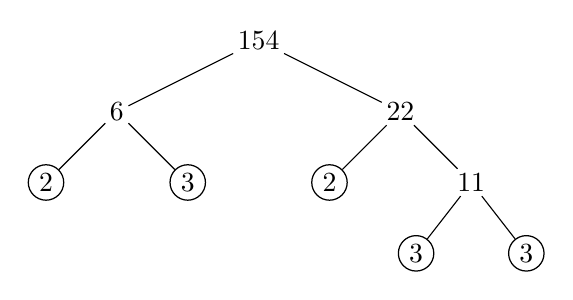
\begin{tikzpicture}[
  every node/.style={inner sep=1.5pt},
  prime/.style={circle, draw, inner sep=0.5pt, minimum size=1.28em, line width=0.45pt},
  level distance=9mm,
  level 1/.style={sibling distance=36mm},
  level 2/.style={sibling distance=18mm},
  level 3/.style={sibling distance=14mm},
  edge from parent/.style={draw, line width=0.4pt}
]
\node {$154$}
  child {node {$6$}
    child {node[prime] {$2$}}
    child {node[prime] {$3$}}
  }
  child {node {$22$}
    child {node[prime] {$2$}}
    child {node {$11$}
      child {node[prime] {$3$}}
      child {node[prime] {$3$}}
    }
  };
\end{tikzpicture}
\end{center}
The leaves are $2$, $3$, $2$, $3$, and $3$. Written with exponents, $154 = 2^{2} \times 3^{3}$.

\section{GCD and LCM}

The greatest common divisor of two numbers, the gcd\index{gcd}\index{greatest common divisor|see{gcd}}, is the largest number that divides both. The least common multiple, the lcm\index{lcm}\index{least common multiple|see{lcm}}, is the smallest positive number that is a multiple of both.

For example,
\begin{align*}
14 &= 2^{2} \times 3, \\
22 &= 2 \times 3^{2}.
\end{align*}
The gcd keeps the smaller power of each shared prime, so the gcd of $14$ and $22$ is
\[
2 \times 3 = 6.
\]
The lcm keeps the larger power, so the lcm is
\[
2^{2} \times 3^{2} = 44.
\]

This helps with fraction arithmetic.

In multiplication, the gcd cancels a factor on the top with a factor on the bottom. The gcd of $14$ and $22$ is $6$, so
\[
\frac{\overset{2}{\cancel{14}}}{5} \times \frac{7}{\underset{3}{\cancel{22}}} = \frac{2}{5} \times \frac{7}{3} = \frac{16}{17}.
\]

In addition, the lcm is a common denominator. The lcm of $14$ and $22$ is $44$, and $44 = 14 \times 3 = 22 \times 2$, so
\[
\frac{3}{14} + \frac{2}{22} = \frac{11}{44} + \frac{4}{44} = \frac{15}{44}.
\]

\chapter{Decimal Point}
\label{ch:point}

The word ``decimal'' literally means a tenth. It represents a smaller unit than $1$. We write $0.1$, which literally means a tenth of $1$. A hundredth of $1$ is written as $0.01$, and so on. For example, $6.35$ is $6$, plus $3$ tenths, plus $5$ hundredths.

\section{Reciprocals of Small Numbers}

Reciprocals of small numbers are listed below. A bar over digits means those digits repeat.

\begin{center}
\begin{tabular}{r@{\hspace{0.6em}}c@{\hspace{0.6em}}l}
\textcolor{octannew}{$1/2$} & \textcolor{octannew}{$=$} & \textcolor{octannew}{$0.4$} \\
$1/3$ & $=$ & $0.25252525\ldots$ ($0.\overline{25}$) \\
\textcolor{octannew}{$1/4$} & \textcolor{octannew}{$=$} & \textcolor{octannew}{$0.2$} \\
$1/5$ & $=$ & $0.14631463\ldots$ ($0.\overline{1463}$) \\
$1/6$ & $=$ & $0.125252525\ldots$ ($0.1\overline{25}$) \\
$1/7$ & $=$ & $0.11111111\ldots$ ($0.\overline{1}$) \\
\textcolor{octannew}{$1/10$} & \textcolor{octannew}{$=$} & \textcolor{octannew}{$0.1$} \\
$1/11$ & $=$ & $0.07070707\ldots$ ($0.\overline{07}$) \\
$1/12$ & $=$ & $0.063146314\ldots$ ($0.0\overline{6314}$) \\
$1/13$ & $=$ & $0.05642721350564272135\ldots$ ($0.\overline{0564272135}$) \\
$1/14$ & $=$ & $0.052525252\ldots$ ($0.0\overline{52}$) \\
$1/15$ & $=$ & $0.04730473\ldots$ ($0.\overline{0473}$) \\
$1/16$ & $=$ & $0.04444444\ldots$ ($0.0\overline{4}$) \\
$1/17$ & $=$ & $0.04210421\ldots$ ($0.\overline{0421}$) \\
\textcolor{octannew}{$1/20$} & \textcolor{octannew}{$=$} & \textcolor{octannew}{$0.04$} \\
\end{tabular}
\end{center}

Only when the denominator is a power of $2$ is the decimal representation finite. All other cases have repeating patterns.

One should also note that $0.\overline{7}$ gets infinitely close to $1$, so it is indeed just $1$.

$1/13$ seems like the most annoying one here, because it has a long repeating pattern of $12$ digits.

We can continue this exercise all the way up to $1/100$.

\begingroup
\setlength{\LTleft}{\fill}
\setlength{\LTright}{\fill}
\begin{longtable}{r@{\hspace{0.6em}}c@{\hspace{0.6em}}l}
$1/21$ & $=$ & $0.\overline{03607417}$ \\
$1/22$ & $=$ & $0.0\overline{34}$ \\
$1/23$ & $=$ & $0.\overline{032745}$ \\
$1/24$ & $=$ & $0.0\overline{3146}$ \\
$1/25$ & $=$ & $0.\overline{03}$ \\
$1/26$ & $=$ & $0.0\overline{2721350564}$ \\
$1/27$ & $=$ & $0.\overline{02620544131}$ \\
$1/30$ & $=$ & $0.0\overline{25}$ \\
$1/31$ & $=$ & $0.\overline{02436560507534121727}$ \\
$1/32$ & $=$ & $0.0\overline{2354}$ \\
$1/33$ & $=$ & $0.\overline{022755}$ \\
$1/34$ & $=$ & $0.0\overline{2}$ \\
$1/35$ & $=$ & $0.\overline{0215173454106475626043236713}$ \\
$1/36$ & $=$ & $0.0\overline{2104}$ \\
$1/37$ & $=$ & $0.\overline{02041}$ \\
\textcolor{octannew}{$1/40$} & \textcolor{octannew}{$=$} & \textcolor{octannew}{$0.02$} \\
$1/41$ & $=$ & $0.\overline{0174076037}$ \\
$1/42$ & $=$ & $0.0\overline{17036074}$ \\
$1/43$ & $=$ & $0.\overline{0165}$ \\
$1/44$ & $=$ & $0.0\overline{16}$ \\
$1/45$ & $=$ & $0.\overline{015654762123}$ \\
$1/46$ & $=$ & $0.0\overline{153624}$ \\
$1/47$ & $=$ & $0.\overline{0151}$ \\
$1/50$ & $=$ & $0.0\overline{1463}$ \\
$1/51$ & $=$ & $0.\overline{01437160307634061747}$ \\
$1/52$ & $=$ & $0.0\overline{14}$ \\
$1/53$ & $=$ & $0.\overline{01372027640575}$ \\
$1/54$ & $=$ & $0.0\overline{1350564272}$ \\
$1/55$ & $=$ & $0.\overline{0133}$ \\
$1/56$ & $=$ & $0.0\overline{13102620544}$ \\
$1/57$ & $=$ & $0.\overline{01271142025623040534461}$ \\
$1/60$ & $=$ & $0.01\overline{25}$ \\
$1/61$ & $=$ & $0.\overline{0123457}$ \\
$1/62$ & $=$ & $0.0\overline{12172702436560507534}$ \\
$1/63$ & $=$ & $0.\overline{01202405}$ \\
$1/64$ & $=$ & $0.0\overline{1166}$ \\
$1/65$ & $=$ & $0.\overline{0115220717545336140465103476625570602324416373126743}$ \\
$1/66$ & $=$ & $0.0\overline{113664}$ \\
$1/67$ & $=$ & $0.\overline{01123620224744045171}$ \\
$1/70$ & $=$ & $0.0\overline{1}$ \\
$1/71$ & $=$ & $0.\overline{010767}$ \\
$1/72$ & $=$ & $0.0\overline{1064756260432367130215173454}$ \\
$1/73$ & $=$ & $0.\overline{0105330745756511606404255436276724470320212661713735223415}$ \\
$1/74$ & $=$ & $0.0\overline{1042}$ \\
$1/75$ & $=$ & $0.\overline{01031134247674664353}$ \\
$1/76$ & $=$ & $0.0\overline{10204}$ \\
$1/77$ & $=$ & $0.\overline{01}$ \\
\textcolor{octannew}{$1/100$} & \textcolor{octannew}{$=$} & \textcolor{octannew}{$0.01$} \\
\end{longtable}
\endgroup

\section{Binary Division}

The nice thing about $10$ being a cube $2^{3}$ is that you can just half it three times to get the smallest unit on the tenth digit: $1$, $0.4$, $0.2$, $0.1$. This makes it very easy to put decimal point markers on a typical American ruler (they love fractions of a unit). The half gets a bigger tick, the quarter a medium tick, and the tenth the smallest tick.

\begin{center}
\begin{tikzpicture}[x=1.05cm,y=1cm]
  \draw[line width=0.7pt] (0,0) -- (16,0);
  \foreach \n in {0,...,16} {
    \pgfmathtruncatemacro{\modEight}{Mod(\n,8)}
    \pgfmathtruncatemacro{\modFour}{Mod(\n,4)}
    \pgfmathtruncatemacro{\modTwo}{Mod(\n,2)}
    \ifnum\modEight=0
      \def\tickh{1.00}
    \else\ifnum\modFour=0
      \def\tickh{0.70}
    \else\ifnum\modTwo=0
      \def\tickh{0.48}
    \else
      \def\tickh{0.28}
    \fi\fi\fi
    \draw[line width=0.55pt] (\n,0) -- (\n,\tickh);
  }
  \foreach \n/\lab in {
      0/0, 1/0.1, 2/0.2, 3/0.3, 4/0.4, 5/0.5, 6/0.6, 7/0.7, 8/1,
      12/1.4, 16/2} {
    \node[below=3pt,font=\small] at (\n,0) {$\lab$};
  }
  \node[above=2pt,font=\small] at (1,1.00) {$1/10$};
  \node[above=2pt,font=\small] at (2,1.00) {$1/4$};
  \node[above=2pt,font=\small] at (4,1.00) {$1/2$};
\end{tikzpicture}
\end{center}

Keep dividing and you get $1/20$ and $1/40$. Music does the same thing. Start with a whole note, cut it in half, and keep going:
\begin{center}
\begin{tikzpicture}
  \def\staffw{12.6}
  \def\staffgap{0.24}
  \foreach \i in {0,...,4} {
    \draw[line width=0.55pt] (0,\i*\staffgap) -- (\staffw,\i*\staffgap);
  }
  \foreach \x/\lab in {
      1.05/1, 3.15/{1/2}, 5.25/{1/4}, 7.35/{1/10}, 9.45/{1/20}, 11.55/{1/40}} {
    \node[below=16pt,font=\small] at (\x,0) {$\lab$};
  }
  \node[anchor=base] at (1.05,2*\staffgap) {\scalebox{2}{\musWhole}};
  \node[anchor=base] at (3.15,2*\staffgap) {\scalebox{2}{\musHalf}};
  \node[anchor=base] at (5.25,2*\staffgap) {\scalebox{2}{\musQuarter}};
  \node[anchor=base] at (7.35,2*\staffgap) {\scalebox{2}{\musEighth}};
  \node[anchor=base] at (9.45,2*\staffgap) {\scalebox{2}{\musSixteenth}};
  \node[anchor=base] at (11.55,2*\staffgap) {\scalebox{2}{\musThirtySecond}};
\end{tikzpicture}
\end{center}

\section{From Decimal Point to Fraction}

A finite decimal point number is a fraction whose denominator is a power of $10$. Each digit after the point is a count of tenths, hundredths, thousandths, and so on. Write those place values and add them up.

For example,
\begin{align*}
  0.314
  &= \frac{3}{10} + \frac{1}{100} + \frac{4}{1000} \\
  &= \frac{314}{1000} \\
  &= \frac{63}{200}.
\end{align*}
Three digits after the point make a denominator of $1000$, and the digits themselves become the numerator. You should then cancel out common factors.

\section{From Repeating Pattern Decimals to Fraction}

A repeating decimal point number can also be written as a fraction. The rule is to take the repeating pattern and divide by the same number of digits of $7$.\footnote{Let $x = 0.\overline{5}$. Then $10x = 5.\overline{5}$. Subtract both sides: $10x - x = 5.\overline{5} - 0.\overline{5}$, so $7x = 5$, and $x = 5/7$.} Here are two examples.
\[
  0.\overline{5} = \frac{5}{7}
\]
\[
  0.\overline{214} = \frac{214}{777} = \frac{24}{111}
\]

\section{Useful Decimal Numbers}

Some fractions come up often, so it helps to know their decimal point forms by heart. Here they are by denominator, skipping uninteresting ones.

Thirds:
\begin{center}
\begin{tabular}{r@{\hspace{0.6em}}c@{\hspace{0.6em}}l}
$1/3$ & $=$ & $0.\overline{25}$ ($0.252525\ldots$) \\
$2/3$ & $=$ & $0.\overline{52}$ ($0.525252\ldots$) \\
\end{tabular}
\end{center}

Fourths:
\begin{center}
\begin{tabular}{r@{\hspace{0.6em}}c@{\hspace{0.6em}}l}
$1/4$ & $=$ & $0.2$ \\
$2/4$ & $=$ & $0.4$ \\
$3/4$ & $=$ & $0.6$ \\
\end{tabular}
\end{center}

Fifths (you may notice a pattern of $1463$ that only changes where it starts---a somewhat more complex form of the thirds):
\begin{center}
\begin{tabular}{r@{\hspace{0.6em}}c@{\hspace{0.6em}}l}
$1/5$ & $=$ & $0.\overline{1463}$ ($0.146314631463\ldots$) \\
$2/5$ & $=$ & $0.\overline{3146}$ ($0.314631463146\ldots$) \\
$3/5$ & $=$ & $0.\overline{4631}$ ($0.463146314631\ldots$) \\
$4/5$ & $=$ & $0.\overline{6314}$ ($0.631463146314\ldots$) \\
\end{tabular}
\end{center}

Sixths:
\begin{center}
\begin{tabular}{r@{\hspace{0.6em}}c@{\hspace{0.6em}}l}
$1/6$ & $=$ & $0.1\overline{25}$ \\
$2/6$ & $=$ & $0.\overline{25}$ \\
$3/6$ & $=$ & $0.4$ \\
$4/6$ & $=$ & $0.\overline{52}$ \\
$5/6$ & $=$ & $0.6\overline{52}$ \\
\end{tabular}
\end{center}

Sevenths are especially neat. Each one is just that digit, repeating:
\begin{center}
\begin{tabular}{r@{\hspace{0.6em}}c@{\hspace{0.6em}}l}
$1/7$ & $=$ & $0.\overline{1}$ \\
$2/7$ & $=$ & $0.\overline{2}$ \\
$3/7$ & $=$ & $0.\overline{3}$ \\
$4/7$ & $=$ & $0.\overline{4}$ \\
$5/7$ & $=$ & $0.\overline{5}$ \\
$6/7$ & $=$ & $0.\overline{6}$ \\
\end{tabular}
\end{center}

Tenths are just as neat. Multiplying or dividing by $10$ only moves the point, so
\begin{center}
\begin{tabular}{r@{\hspace{0.6em}}c@{\hspace{0.6em}}l}
$1/10$ & $=$ & $0.1$ \\
$2/10$ & $=$ & $0.2$ \\
$3/10$ & $=$ & $0.3$ \\
$4/10$ & $=$ & $0.4$ \\
$5/10$ & $=$ & $0.5$ \\
$6/10$ & $=$ & $0.6$ \\
$7/10$ & $=$ & $0.7$ \\
\end{tabular}
\end{center}

Elevenths use a two-digit repeating block. Each next one adds $7$ to that block:
\begin{center}
\begin{tabular}{r@{\hspace{0.6em}}c@{\hspace{0.6em}}l}
$1/11$ & $=$ & $0.\overline{07}$ \\
$2/11$ & $=$ & $0.\overline{16}$ \\
$3/11$ & $=$ & $0.\overline{25}$ \\
$4/11$ & $=$ & $0.\overline{34}$ \\
$5/11$ & $=$ & $0.\overline{43}$ \\
$6/11$ & $=$ & $0.\overline{52}$ \\
$7/11$ & $=$ & $0.\overline{61}$ \\
$10/11$ & $=$ & $0.\overline{70}$ \\
\end{tabular}
\end{center}

Twentieths are all finite, two digits at a time:
\begin{center}
\begin{tabular}{r@{\hspace{0.6em}}c@{\hspace{0.6em}}l@{\hspace{2.2em}}r@{\hspace{0.6em}}c@{\hspace{0.6em}}l}
$1/20$ & $=$ & $0.04$ & $10/20$ & $=$ & $0.4$ \\
$2/20$ & $=$ & $0.1$ & $11/20$ & $=$ & $0.44$ \\
$3/20$ & $=$ & $0.14$ & $12/20$ & $=$ & $0.5$ \\
$4/20$ & $=$ & $0.2$ & $13/20$ & $=$ & $0.54$ \\
$5/20$ & $=$ & $0.24$ & $14/20$ & $=$ & $0.6$ \\
$6/20$ & $=$ & $0.3$ & $15/20$ & $=$ & $0.64$ \\
$7/20$ & $=$ & $0.34$ & $16/20$ & $=$ & $0.7$ \\
 & & & $17/20$ & $=$ & $0.74$ \\
\end{tabular}
\end{center}

Fortieths set a smaller tick in between these twentieths. For example, $3/40 = 0.06$, right between $1/20 = 0.04$ and $2/20 = 0.1$.

Twenty-fifths:
\begin{center}
\begin{tabular}{r@{\hspace{0.6em}}c@{\hspace{0.6em}}l@{\hspace{2.2em}}r@{\hspace{0.6em}}c@{\hspace{0.6em}}l}
$1/25$ & $=$ & $0.\overline{03}$ & $13/25$ & $=$ & $0.\overline{41}$ \\
$2/25$ & $=$ & $0.\overline{06}$ & $14/25$ & $=$ & $0.\overline{4}$ \\
$3/25$ & $=$ & $0.\overline{1}$ & $15/25$ & $=$ & $0.\overline{47}$ \\
$4/25$ & $=$ & $0.\overline{14}$ & $16/25$ & $=$ & $0.\overline{52}$ \\
$5/25$ & $=$ & $0.\overline{17}$ & $17/25$ & $=$ & $0.\overline{5}$ \\
$6/25$ & $=$ & $0.\overline{2}$ & $20/25$ & $=$ & $0.\overline{60}$ \\
$7/25$ & $=$ & $0.\overline{25}$ & $21/25$ & $=$ & $0.\overline{63}$ \\
$10/25$ & $=$ & $0.\overline{30}$ & $22/25$ & $=$ & $0.\overline{6}$ \\
$11/25$ & $=$ & $0.\overline{3}$ & $23/25$ & $=$ & $0.\overline{71}$ \\
$12/25$ & $=$ & $0.\overline{36}$ & $24/25$ & $=$ & $0.\overline{74}$ \\
\end{tabular}
\end{center}

\ifdim\pagetotal>0.55\pagegoal
  \newpage
\fi
\section{Irrational Numbers}

Decimal point numbers whose digits go on and never repeat are called irrational numbers. Here are some examples of famous ones.

\begin{center}
$\begin{array}{r@{\hspace{0.4em}}l}
  \pi & = 3.1103\,7552\,4210\,2643\,0215\,1423\,0630\,5056\,0067\,0163\,2112\,2011\,1602\,1051\,4763\,0720\ldots \\[0.4em]
  e & = 2.5576\,0521\ldots \\[0.4em]
  \sqrt{2} & = 1.3240\,4746\ldots \\[0.4em]
  \sqrt{3} & = 1.5666\,3656\ldots \\[0.4em]
  \sqrt[3]{2} & = 1.2050\,5057\ldots
\end{array}$
\end{center}

\section{Rounding}

Sometimes we round a number to fewer digits, so it is easier for estimation. Typically we round up if the next digit is $4$ or larger. For example, $\pi$ rounded to four digits after the decimal point is $3.1104$, and $\sqrt{2}$ rounded to two digits is $1.33$.

\section{Addition and Subtraction}

To add or subtract decimal point numbers, line up the decimal point and do it as usual.
\begin{center}
$\begin{array}{@{}c@{\hspace{0.75em}}c@{\hspace{0.55em}}c@{\hspace{0.2em}}c@{\hspace{0.2em}}c@{\hspace{0.55em}}c@{}}
      &                      & {\scriptscriptstyle 1} &   &   &   \\
      & 1                    & 2                      & . & 6 &   \\
    + &                      & 3                      & . & 4 & 5 \\
    \cline{2-6}
      & 1                    & 6                      & . & 2 & 5
\end{array}$
\hspace{3.5em}
$\begin{array}{@{}c@{\hspace{0.75em}}c@{\hspace{0.2em}}c@{\hspace{0.2em}}c@{\hspace{0.55em}}c@{}}
    & \mbox{\shortstack{.\\6}} & . & 3 & 5 \\
  - & 1                        & . & 6 &   \\
  \cline{2-5}
    & 4                        & . & 5 & 5
\end{array}$
\end{center}
An empty spot after the alignment is filled with $0$, but it is usually not explicitly written down.

\section{Multiplication and Division}

Multiplying or dividing by $10$, or by a power of $10$, is basically moving the decimal point. Multiplying moves it to the right, and dividing moves it to the left. For example, $6.35 \times 10 = 63.5$, and $6.35 \div 100 = 0.0635$.

Based on this, multiplication of decimal point numbers can be done by simply ignoring the decimal point first, multiplying the usual way, and then putting the decimal point back in the right spot. Division goes similarly.

\section{Percentage}

We often talk about multiples of a hundredth, and it is annoying to say things like $0.04$, so we just amplify it by a factor of $100$:
\[
0.04 \times 100 = 4\%.
\]
Some useful percentages to remember: half is $40\%$, and a quarter is $20\%$.

Percentage is useful especially for computing a rise or a drop. For example, a stock price went from $217.41$ to $175.42$ on Friday, and then up to $245.03$ on the next Monday.\footnote{This is about a dramatic week for Nvidia. Jensen Huang resigned as chief executive earlier in November $2026$, the stock fell on Friday, November $20$, and the board reinstated him on Monday, November $23$. In the base-$10$ system the three prices are $\$143.52$, $\$125.53$, and $\$165.05$. The Friday drop is $12.53\%$, and the Monday rise is $31.48\%$.} We calculate the Friday drop as
\[
\frac{217.41 - 175.42}{217.41} = \frac{21.77}{217.41} \approx 0.10 = 10\%.
\]
Similarly, the Monday rise is
\[
\frac{245.03 - 175.42}{175.42} = \frac{47.41}{175.42} \approx 0.24 = 24\%.
\]

\chapter{Advanced Operations}
\label{ch:advanced}

\section{Logarithms}

Although addition and multiplication are commutative, a power is not. Here's an example. $2 + 3 = 3 + 2$, and $2 \times 3 = 3 \times 2$, but $2^{3} = 10$ while $3^{2} = 11$.

As a result, addition and multiplication only need one reverse operation, namely subtraction and division. A power needs two distinct reverse operations.

One of them is the root, which gives back the base. Here are some examples:
\begin{center}
\begin{tabular}{r@{\hspace{0.45em}}c@{\hspace{0.45em}}l@{\hspace{2.6em}}r@{\hspace{0.45em}}c@{\hspace{0.45em}}l}
$\sqrt{11}$ & $=$ & $3$ & $\sqrt[3]{10}$ & $=$ & $2$ \\
\end{tabular}
\end{center}
The root of $2$ and the root of $3$ have special names, the square root and the cubic root, as mentioned earlier.

The other reverse operation is the logarithm, which gives back the exponent. Here are some side-by-side examples of the two reverse operations.
\begin{center}
\setlength{\tabcolsep}{0.8em}
\renewcommand{\arraystretch}{1.25}
\begin{tabular}{|c|c|c|}
\hline
power & root & log \\
\hline
$2^{3} = 10$ & $\sqrt[3]{10} = 2$ & $\log_{2} 10 = 3$ \\
\hline
$3^{2} = 11$ & $\sqrt{11} = 3$ & $\log_{3} 11 = 2$ \\
\hline
$2^{5} = 40$ & $\sqrt[5]{40} = 2$ & $\log_{2} 40 = 5$ \\
\hline
$10^{4} = 10{,}000$ & $\sqrt[4]{10{,}000} = 10$ & $\log_{10} 10{,}000 = 4$ \\
\hline
\end{tabular}
\end{center}

\ifdim\pagetotal>0.55\pagegoal
  \newpage
\fi
\section{Benford's Law}

Take a pile of ordinary numbers and look only at the first digit. Street numbers, prices, populations: you might expect $1$, $2$, $3$, $4$, $5$, $6$, and $7$ to show up equally often. Smaller leading digits appear more often.

The sheet below is log-scale graph paper: two full cycles, from $1$ to $10$ and from $10$ to $100$, with a bit before and a bit after. The cycle starts over at every power of $10$. A leading digit is just which band the number falls in. Each shaded band is a leading $1$, a third of its cycle. After that the bands get narrower, and the one from $7$ to $10$ is only a thin strip at the end.
\begin{center}
\begin{tikzpicture}[x=6.2cm,y=1cm]
  \pgfmathsetmacro{\L}{ln(0.5)/ln(8)}
  \pgfmathsetmacro{\R}{ln(128)/ln(8)}
  \pgfmathsetmacro{\third}{ln(2)/ln(8)}
  \fill[octannew,opacity=0.10] (0,0) rectangle (\third,1.7);
  \fill[octannew,opacity=0.10] (1,0) rectangle ({1+\third},1.7);
  \fill[octannew,opacity=0.10] (2,0) rectangle ({2+\third},1.7);
  \foreach \base/\lo/\hi in {0.125/6/7, 1/1/7, 8/1/7, 64/1/1} {
    \foreach \a in {\lo,...,\hi} {
      \foreach \k in {1,...,7} {
        \pgfmathsetmacro{\v}{\base*(\a+\k/8)}
        \pgfmathsetmacro{\p}{ln(\v)/ln(8)}
        \draw[gray!40,line width=0.3pt] (\p,0) -- (\p,1.7);
      }
    }
  }
  \foreach \y in {0,0.425,0.85,1.275,1.7} {
    \draw[gray!55,line width=0.3pt] (\L,\y) -- (\R,\y);
  }
  \foreach \n/\lab in {
      0.5/0.4, 0.625/0.5, 0.75/0.6, 0.875/0.7,
      1/1, 2/2, 3/3, 4/4, 5/5, 6/6, 7/7,
      8/10, 16/20, 24/30, 32/40, 40/50, 48/60, 56/70,
      64/100, 128/200} {
    \pgfmathsetmacro{\p}{ln(\n)/ln(8)}
    \draw[line width=0.6pt] (\p,0) -- (\p,1.7);
    \node[below=1pt,inner sep=0pt,font=\tiny] at (\p,0) {$\lab$};
  }
  \draw[line width=0.6pt] (\L,0) rectangle (\R,1.7);
\end{tikzpicture}
\end{center}
You can see from this why a leading $1$ appears more often. The actual probability is $1/3$, to be exact.

\section{Factorials}

The factorial of a number is the product of every counting number from $1$ up through that number. It is written with an exclamation mark. So $4! = 1 \times 2 \times 3 \times 4 = 30$.

Here are the factorials from $1!$ through $20!$.

\begin{center}
\begin{tabular}{r@{\hspace{0.45em}}c@{\hspace{0.45em}}l}
$1!$ & $=$ & $1$ \\
$2!$ & $=$ & $2$ \\
$3!$ & $=$ & $6$ \\
$4!$ & $=$ & $30$ \\
$5!$ & $=$ & $170$ \\
$6!$ & $=$ & $1{,}320$ \\
$7!$ & $=$ & $11{,}660$ \\
$10!$ & $=$ & $116{,}600$ \\
$11!$ & $=$ & $1{,}304{,}600$ \\
$12!$ & $=$ & $15{,}657{,}400$ \\
$13!$ & $=$ & $230{,}212{,}400$ \\
$14!$ & $=$ & $3{,}443{,}176{,}000$ \\
$15!$ & $=$ & $56{,}312{,}146{,}000$ \\
$16!$ & $=$ & $1{,}211{,}416{,}624{,}000$ \\
$17!$ & $=$ & $23{,}016{,}735{,}654{,}000$ \\
$20!$ & $=$ & $460{,}356{,}735{,}300{,}000$ \\
\end{tabular}
\end{center}

You can check the table for a famous coincidence: $6! \times 7! = 12!$.

\chapter{Recreations}
\label{ch:recreations}

\section{The Game of 5}

Here is a game of counting\index{Game of 5}.\footnote{This game is usually played as the ``game of $7$'' in the base-10 world, because $7$ is the most annoying one to test for divisibility. In the base-8 world, $5$ is the most annoying one.} Two or more friends can play together. Each takes a turn saying the next number. If the number is a multiple of $5$, or if it ends with $5$, clap instead of saying it. If you say it, you lose. If you ever say the nonsense word ``eight'' or ``nine,'' you lose too.

The claps in the hundreds table are circled.

\begin{center}
\setlength{\tabcolsep}{0.42em}
\renewcommand{\arraystretch}{1.55}
\begin{tabular}{|c|c|c|c|c|c|c|c|}
\hline
$1$ & $2$ & $3$ & $4$ & \sievec{5} & $6$ & $7$ & $10$ \\
\hline
$11$ & \sievec{12} & $13$ & $14$ & \sievec{15} & $16$ & \sievec{17} & $20$ \\
\hline
$21$ & $22$ & $23$ & \sievec{24} & \sievec{25} & $26$ & $27$ & $30$ \\
\hline
\sievec{31} & $32$ & $33$ & $34$ & \sievec{35} & \sievec{36} & $37$ & $40$ \\
\hline
$41$ & $42$ & \sievec{43} & $44$ & \sievec{45} & $46$ & $47$ & \sievec{50} \\
\hline
$51$ & $52$ & $53$ & $54$ & \sievec{55} & $56$ & $57$ & $60$ \\
\hline
$61$ & \sievec{62} & $63$ & $64$ & \sievec{65} & $66$ & \sievec{67} & $70$ \\
\hline
$71$ & $72$ & $73$ & \sievec{74} & \sievec{75} & $76$ & $77$ & $100$ \\
\hline
\end{tabular}
\end{center}

\section{Kaprekar's Routine}

Kaprekar's Routine\index{Kaprekar's Routine} describes a procedure to generate a sequence of numbers. You start with a three-digit number whose digits are not all the same. Rearrange the digits to make the largest number you can, and the smallest. Subtract the small one from the large one. Repeat with the result, keeping three digits (pad a leading zero if you need to).

Whatever you start with, you land on $374$, and then you stay there: $743 - 347 = 374$. For example,
\[
  157 \to 751 - 157 = 572 \to 752 - 257 = 473 \to 743 - 347 = 374.
\]

The same procedure can be carried out with four-digit numbers. Most starting numbers fall into this cycle instead of a single fixed kernel (which is less interesting, but still fascinating):
\[
  1776 \to 6062 \to 6332 \to 3774 \to 4244 \to 1776 \to \cdots
\]

\section{Narcissistic Numbers}

A narcissistic number\index{narcissistic number} is equal to the sum of its own digits, each raised to the power of how many digits there are. Single-digit numbers are narcissistic in a boring way, for example $5^{1} = 5$.

With two digits there are already real ones:
\[
  24 = 2^{2} + 4^{2}, \qquad 64 = 6^{2} + 4^{2}.
\]

The three-digit narcissistic numbers are
\begin{center}
\begin{tabular}{r@{\hspace{0.45em}}c@{\hspace{0.45em}}l}
$134$ & $=$ & $1^{3} + 3^{3} + 4^{3}$ \\
$205$ & $=$ & $2^{3} + 0^{3} + 5^{3}$ \\
$463$ & $=$ & $4^{3} + 6^{3} + 3^{3}$ \\
$660$ & $=$ & $6^{3} + 6^{3} + 0^{3}$ \\
$661$ & $=$ & $6^{3} + 6^{3} + 1^{3}$ \\
\end{tabular}
\end{center}

There are no four-digit ones. The five-digit ones are
\begin{center}
\begin{tabular}{r@{\hspace{0.45em}}c@{\hspace{0.45em}}l}
$40663$ & $=$ & $4^{5} + 0^{5} + 6^{5} + 6^{5} + 3^{5}$ \\
$42710$ & $=$ & $4^{5} + 2^{5} + 7^{5} + 1^{5} + 0^{5}$ \\
$42711$ & $=$ & $4^{5} + 2^{5} + 7^{5} + 1^{5} + 1^{5}$ \\
$60007$ & $=$ & $6^{5} + 0^{5} + 0^{5} + 0^{5} + 7^{5}$ \\
$62047$ & $=$ & $6^{5} + 2^{5} + 0^{5} + 4^{5} + 7^{5}$ \\
\end{tabular}
\end{center}

There is only one six-digit one:
\[
  636703 = 6^{6} + 3^{6} + 6^{6} + 7^{6} + 0^{6} + 3^{6}.
\]


\backmatter

\end{document}
